\documentclass[twoside]{book}

% Packages required by doxygen
\usepackage{fixltx2e}
\usepackage{calc}
\usepackage{doxygen}
\usepackage[export]{adjustbox} % also loads graphicx
\usepackage{graphicx}
\usepackage[utf8]{inputenc}
\usepackage{makeidx}
\usepackage{multicol}
\usepackage{multirow}
\PassOptionsToPackage{warn}{textcomp}
\usepackage{textcomp}
\usepackage[nointegrals]{wasysym}
\usepackage[table]{xcolor}

% Font selection
\usepackage[T1]{fontenc}
\usepackage[scaled=.90]{helvet}
\usepackage{courier}
\usepackage{amssymb}
\usepackage{sectsty}
\renewcommand{\familydefault}{\sfdefault}
\allsectionsfont{%
  \fontseries{bc}\selectfont%
  \color{darkgray}%
}
\renewcommand{\DoxyLabelFont}{%
  \fontseries{bc}\selectfont%
  \color{darkgray}%
}
\newcommand{\+}{\discretionary{\mbox{\scriptsize$\hookleftarrow$}}{}{}}

% Page & text layout
\usepackage{geometry}
\geometry{%
  a4paper,%
  top=2.5cm,%
  bottom=2.5cm,%
  left=2.5cm,%
  right=2.5cm%
}
\tolerance=750
\hfuzz=15pt
\hbadness=750
\setlength{\emergencystretch}{15pt}
\setlength{\parindent}{0cm}
\setlength{\parskip}{3ex plus 2ex minus 2ex}
\makeatletter
\renewcommand{\paragraph}{%
  \@startsection{paragraph}{4}{0ex}{-1.0ex}{1.0ex}{%
    \normalfont\normalsize\bfseries\SS@parafont%
  }%
}
\renewcommand{\subparagraph}{%
  \@startsection{subparagraph}{5}{0ex}{-1.0ex}{1.0ex}{%
    \normalfont\normalsize\bfseries\SS@subparafont%
  }%
}
\makeatother

% Headers & footers
\usepackage{fancyhdr}
\pagestyle{fancyplain}
\fancyhead[LE]{\fancyplain{}{\bfseries\thepage}}
\fancyhead[CE]{\fancyplain{}{}}
\fancyhead[RE]{\fancyplain{}{\bfseries\leftmark}}
\fancyhead[LO]{\fancyplain{}{\bfseries\rightmark}}
\fancyhead[CO]{\fancyplain{}{}}
\fancyhead[RO]{\fancyplain{}{\bfseries\thepage}}
\fancyfoot[LE]{\fancyplain{}{}}
\fancyfoot[CE]{\fancyplain{}{}}
\fancyfoot[RE]{\fancyplain{}{\bfseries\scriptsize Generated by Doxygen }}
\fancyfoot[LO]{\fancyplain{}{\bfseries\scriptsize Generated by Doxygen }}
\fancyfoot[CO]{\fancyplain{}{}}
\fancyfoot[RO]{\fancyplain{}{}}
\renewcommand{\footrulewidth}{0.4pt}
\renewcommand{\chaptermark}[1]{%
  \markboth{#1}{}%
}
\renewcommand{\sectionmark}[1]{%
  \markright{\thesection\ #1}%
}

% Indices & bibliography
\usepackage{natbib}
\usepackage[titles]{tocloft}
\setcounter{tocdepth}{3}
\setcounter{secnumdepth}{5}
\makeindex

% Hyperlinks (required, but should be loaded last)
\usepackage{ifpdf}
\ifpdf
  \usepackage[pdftex,pagebackref=true]{hyperref}
\else
  \usepackage[ps2pdf,pagebackref=true]{hyperref}
\fi
\hypersetup{%
  colorlinks=true,%
  linkcolor=blue,%
  citecolor=blue,%
  unicode%
}

% Custom commands
\newcommand{\clearemptydoublepage}{%
  \newpage{\pagestyle{empty}\cleardoublepage}%
}

\usepackage{caption}
\captionsetup{labelsep=space,justification=centering,font={bf},singlelinecheck=off,skip=4pt,position=top}

%===== C O N T E N T S =====

\begin{document}

% Titlepage & ToC
\hypersetup{pageanchor=false,
             bookmarksnumbered=true,
             pdfencoding=unicode
            }
\pagenumbering{alph}
\begin{titlepage}
\vspace*{7cm}
\begin{center}%
{\Large necasy \\[1ex]\large 0.\+1 }\\
\vspace*{1cm}
{\large Generated by Doxygen 1.8.13}\\
\end{center}
\end{titlepage}
\clearemptydoublepage
\pagenumbering{roman}
\tableofcontents
\clearemptydoublepage
\pagenumbering{arabic}
\hypersetup{pageanchor=true}

%--- Begin generated contents ---
\chapter{Hierarchical Index}
\section{Class Hierarchy}
This inheritance list is sorted roughly, but not completely, alphabetically\+:\begin{DoxyCompactList}
\item \contentsline{section}{Camera}{\pageref{classCamera}}{}
\item \contentsline{section}{rapidcsv\+:\+:Converter$<$ T $>$}{\pageref{classrapidcsv_1_1Converter}}{}
\item \contentsline{section}{rapidcsv\+:\+:Converter\+Params}{\pageref{structrapidcsv_1_1ConverterParams}}{}
\item \contentsline{section}{rapidcsv\+:\+:Document}{\pageref{classrapidcsv_1_1Document}}{}
\item exception\begin{DoxyCompactList}
\item \contentsline{section}{rapidcsv\+:\+:no\+\_\+converter}{\pageref{classrapidcsv_1_1no__converter}}{}
\end{DoxyCompactList}
\item \contentsline{section}{rapidcsv\+:\+:Label\+Params}{\pageref{structrapidcsv_1_1LabelParams}}{}
\item \contentsline{section}{rapidcsv\+:\+:Line\+Reader\+Params}{\pageref{structrapidcsv_1_1LineReaderParams}}{}
\item \contentsline{section}{Necasy}{\pageref{classNecasy}}{}
\item \contentsline{section}{rapidcsv\+:\+:Separator\+Params}{\pageref{structrapidcsv_1_1SeparatorParams}}{}
\end{DoxyCompactList}

\chapter{Class Index}
\section{Class List}
Here are the classes, structs, unions and interfaces with brief descriptions\+:\begin{DoxyCompactList}
\item\contentsline{section}{\hyperlink{classNecasy}{Necasy} \\*Main class for the system }{\pageref{classNecasy}}{}
\end{DoxyCompactList}

\chapter{Class Documentation}
\hypertarget{classCamera}{}\section{Camera Class Reference}
\label{classCamera}\index{Camera@{Camera}}


Class for a network camera.  




{\ttfamily \#include $<$camera.\+hpp$>$}

\subsection*{Public Member Functions}
\begin{DoxyCompactItemize}
\item 
\mbox{\Hypertarget{classCamera_a18f3f52598d6db329356be7ec0bd2a9d}\label{classCamera_a18f3f52598d6db329356be7ec0bd2a9d}} 
{\bfseries Camera} (std\+::string name, std\+::string stream, unsigned int id)
\item 
\mbox{\Hypertarget{classCamera_ad66ff7f06d23b01a3a442c3019af22ce}\label{classCamera_ad66ff7f06d23b01a3a442c3019af22ce}} 
void {\bfseries Capture} ()
\item 
\mbox{\Hypertarget{classCamera_ae4337f38ed32ef67067264f2665c883f}\label{classCamera_ae4337f38ed32ef67067264f2665c883f}} 
void {\bfseries Record} ()
\end{DoxyCompactItemize}


\subsection{Detailed Description}
Class for a network camera. 

This class implements the functionalities of a network camera added to the system.


\begin{DoxyParams}{Parameters}
{\em camera\+\_\+stream} & The address of a camera stream \\
\hline
\end{DoxyParams}


The documentation for this class was generated from the following files\+:\begin{DoxyCompactItemize}
\item 
include/camera.\+hpp\item 
src/camera.\+cpp\end{DoxyCompactItemize}

\hypertarget{classrapidcsv_1_1Converter}{}\section{rapidcsv\+:\+:Converter$<$ T $>$ Class Template Reference}
\label{classrapidcsv_1_1Converter}\index{rapidcsv\+::\+Converter$<$ T $>$@{rapidcsv\+::\+Converter$<$ T $>$}}


Class providing conversion to/from numerical datatypes and strings. Only intended for rapidcsv internal usage, but exposed externally to allow specialization for custom datatype conversions.  




{\ttfamily \#include $<$rapidcsv.\+h$>$}

\subsection*{Public Member Functions}
\begin{DoxyCompactItemize}
\item 
\hyperlink{classrapidcsv_1_1Converter_a8f7de9557f32e24abb022bc9d52ae2e2}{Converter} (const \hyperlink{structrapidcsv_1_1ConverterParams}{Converter\+Params} \&p\+Converter\+Params)
\begin{DoxyCompactList}\small\item\em Constructor. \end{DoxyCompactList}\item 
void \hyperlink{classrapidcsv_1_1Converter_a114b87c39563c7777ad79fa8eb50c8e5}{To\+Str} (const T \&p\+Val, std\+::string \&p\+Str) const
\begin{DoxyCompactList}\small\item\em Converts numerical value to string representation. \end{DoxyCompactList}\item 
void \hyperlink{classrapidcsv_1_1Converter_a827c54e8cbe86cdb8e315d3382dfcbba}{To\+Val} (const std\+::string \&p\+Str, T \&p\+Val) const
\begin{DoxyCompactList}\small\item\em Converts string holding a numerical value to numerical datatype representation. \end{DoxyCompactList}\item 
{\footnotesize template$<$$>$ }\\void \hyperlink{classrapidcsv_1_1Converter_ae3c2d87f4e7cb9d09d4ecdd23419449c}{To\+Str} (const std\+::string \&p\+Val, std\+::string \&p\+Str) const
\begin{DoxyCompactList}\small\item\em Specialized implementation handling string to string conversion. \end{DoxyCompactList}\item 
{\footnotesize template$<$$>$ }\\void \hyperlink{classrapidcsv_1_1Converter_aa038d308c460903344c0c2ebc5251537}{To\+Val} (const std\+::string \&p\+Str, std\+::string \&p\+Val) const
\begin{DoxyCompactList}\small\item\em Specialized implementation handling string to string conversion. \end{DoxyCompactList}\end{DoxyCompactItemize}


\subsection{Detailed Description}
\subsubsection*{template$<$typename T$>$\newline
class rapidcsv\+::\+Converter$<$ T $>$}

Class providing conversion to/from numerical datatypes and strings. Only intended for rapidcsv internal usage, but exposed externally to allow specialization for custom datatype conversions. 

\subsection{Constructor \& Destructor Documentation}
\mbox{\Hypertarget{classrapidcsv_1_1Converter_a8f7de9557f32e24abb022bc9d52ae2e2}\label{classrapidcsv_1_1Converter_a8f7de9557f32e24abb022bc9d52ae2e2}} 
\index{rapidcsv\+::\+Converter@{rapidcsv\+::\+Converter}!Converter@{Converter}}
\index{Converter@{Converter}!rapidcsv\+::\+Converter@{rapidcsv\+::\+Converter}}
\subsubsection{\texorpdfstring{Converter()}{Converter()}}
{\footnotesize\ttfamily template$<$typename T$>$ \\
\hyperlink{classrapidcsv_1_1Converter}{rapidcsv\+::\+Converter}$<$ T $>$\+::\hyperlink{classrapidcsv_1_1Converter}{Converter} (\begin{DoxyParamCaption}\item[{const \hyperlink{structrapidcsv_1_1ConverterParams}{Converter\+Params} \&}]{p\+Converter\+Params }\end{DoxyParamCaption})\hspace{0.3cm}{\ttfamily [inline]}}



Constructor. 


\begin{DoxyParams}{Parameters}
{\em p\+Converter\+Params} & specifies how conversion of non-\/numerical values to numerical datatype shall be handled. \\
\hline
\end{DoxyParams}


\subsection{Member Function Documentation}
\mbox{\Hypertarget{classrapidcsv_1_1Converter_a114b87c39563c7777ad79fa8eb50c8e5}\label{classrapidcsv_1_1Converter_a114b87c39563c7777ad79fa8eb50c8e5}} 
\index{rapidcsv\+::\+Converter@{rapidcsv\+::\+Converter}!To\+Str@{To\+Str}}
\index{To\+Str@{To\+Str}!rapidcsv\+::\+Converter@{rapidcsv\+::\+Converter}}
\subsubsection{\texorpdfstring{To\+Str()}{ToStr()}\hspace{0.1cm}{\footnotesize\ttfamily [1/2]}}
{\footnotesize\ttfamily template$<$typename T$>$ \\
void \hyperlink{classrapidcsv_1_1Converter}{rapidcsv\+::\+Converter}$<$ T $>$\+::To\+Str (\begin{DoxyParamCaption}\item[{const T \&}]{p\+Val,  }\item[{std\+::string \&}]{p\+Str }\end{DoxyParamCaption}) const\hspace{0.3cm}{\ttfamily [inline]}}



Converts numerical value to string representation. 


\begin{DoxyParams}{Parameters}
{\em p\+Val} & numerical value \\
\hline
{\em p\+Str} & output string \\
\hline
\end{DoxyParams}
\mbox{\Hypertarget{classrapidcsv_1_1Converter_ae3c2d87f4e7cb9d09d4ecdd23419449c}\label{classrapidcsv_1_1Converter_ae3c2d87f4e7cb9d09d4ecdd23419449c}} 
\index{rapidcsv\+::\+Converter@{rapidcsv\+::\+Converter}!To\+Str@{To\+Str}}
\index{To\+Str@{To\+Str}!rapidcsv\+::\+Converter@{rapidcsv\+::\+Converter}}
\subsubsection{\texorpdfstring{To\+Str()}{ToStr()}\hspace{0.1cm}{\footnotesize\ttfamily [2/2]}}
{\footnotesize\ttfamily template$<$$>$ \\
void \hyperlink{classrapidcsv_1_1Converter}{rapidcsv\+::\+Converter}$<$ std\+::string $>$\+::To\+Str (\begin{DoxyParamCaption}\item[{const std\+::string \&}]{p\+Val,  }\item[{std\+::string \&}]{p\+Str }\end{DoxyParamCaption}) const\hspace{0.3cm}{\ttfamily [inline]}}



Specialized implementation handling string to string conversion. 


\begin{DoxyParams}{Parameters}
{\em p\+Val} & string \\
\hline
{\em p\+Str} & string \\
\hline
\end{DoxyParams}
\mbox{\Hypertarget{classrapidcsv_1_1Converter_a827c54e8cbe86cdb8e315d3382dfcbba}\label{classrapidcsv_1_1Converter_a827c54e8cbe86cdb8e315d3382dfcbba}} 
\index{rapidcsv\+::\+Converter@{rapidcsv\+::\+Converter}!To\+Val@{To\+Val}}
\index{To\+Val@{To\+Val}!rapidcsv\+::\+Converter@{rapidcsv\+::\+Converter}}
\subsubsection{\texorpdfstring{To\+Val()}{ToVal()}\hspace{0.1cm}{\footnotesize\ttfamily [1/2]}}
{\footnotesize\ttfamily template$<$typename T$>$ \\
void \hyperlink{classrapidcsv_1_1Converter}{rapidcsv\+::\+Converter}$<$ T $>$\+::To\+Val (\begin{DoxyParamCaption}\item[{const std\+::string \&}]{p\+Str,  }\item[{T \&}]{p\+Val }\end{DoxyParamCaption}) const\hspace{0.3cm}{\ttfamily [inline]}}



Converts string holding a numerical value to numerical datatype representation. 


\begin{DoxyParams}{Parameters}
{\em p\+Val} & numerical value \\
\hline
{\em p\+Str} & output string \\
\hline
\end{DoxyParams}
\mbox{\Hypertarget{classrapidcsv_1_1Converter_aa038d308c460903344c0c2ebc5251537}\label{classrapidcsv_1_1Converter_aa038d308c460903344c0c2ebc5251537}} 
\index{rapidcsv\+::\+Converter@{rapidcsv\+::\+Converter}!To\+Val@{To\+Val}}
\index{To\+Val@{To\+Val}!rapidcsv\+::\+Converter@{rapidcsv\+::\+Converter}}
\subsubsection{\texorpdfstring{To\+Val()}{ToVal()}\hspace{0.1cm}{\footnotesize\ttfamily [2/2]}}
{\footnotesize\ttfamily template$<$$>$ \\
void \hyperlink{classrapidcsv_1_1Converter}{rapidcsv\+::\+Converter}$<$ std\+::string $>$\+::To\+Val (\begin{DoxyParamCaption}\item[{const std\+::string \&}]{p\+Str,  }\item[{std\+::string \&}]{p\+Val }\end{DoxyParamCaption}) const\hspace{0.3cm}{\ttfamily [inline]}}



Specialized implementation handling string to string conversion. 


\begin{DoxyParams}{Parameters}
{\em p\+Val} & string \\
\hline
{\em p\+Str} & string \\
\hline
\end{DoxyParams}


The documentation for this class was generated from the following file\+:\begin{DoxyCompactItemize}
\item 
include/rapidcsv.\+h\end{DoxyCompactItemize}

\hypertarget{structrapidcsv_1_1ConverterParams}{}\section{rapidcsv\+:\+:Converter\+Params Struct Reference}
\label{structrapidcsv_1_1ConverterParams}\index{rapidcsv\+::\+Converter\+Params@{rapidcsv\+::\+Converter\+Params}}


Datastructure holding parameters controlling how invalid numbers (including empty strings) should be handled.  




{\ttfamily \#include $<$rapidcsv.\+h$>$}

\subsection*{Public Member Functions}
\begin{DoxyCompactItemize}
\item 
\hyperlink{structrapidcsv_1_1ConverterParams_a9ce85a6fd120b3ecb08c29e2727cd52e}{Converter\+Params} (const bool p\+Has\+Default\+Converter=false, const long double p\+Default\+Float=std\+::numeric\+\_\+limits$<$ long double $>$\+::signaling\+\_\+\+NaN(), const long long p\+Default\+Integer=0, const bool p\+Numeric\+Locale=true)
\begin{DoxyCompactList}\small\item\em Constructor. \end{DoxyCompactList}\end{DoxyCompactItemize}
\subsection*{Public Attributes}
\begin{DoxyCompactItemize}
\item 
\mbox{\Hypertarget{structrapidcsv_1_1ConverterParams_acc9b157c2646d342e42467813e5972d3}\label{structrapidcsv_1_1ConverterParams_acc9b157c2646d342e42467813e5972d3}} 
bool \hyperlink{structrapidcsv_1_1ConverterParams_acc9b157c2646d342e42467813e5972d3}{m\+Has\+Default\+Converter}
\begin{DoxyCompactList}\small\item\em specifies if conversion of non-\/numerical strings shall be converted to a default numerical value, instead of causing an exception to be thrown (default). \end{DoxyCompactList}\item 
\mbox{\Hypertarget{structrapidcsv_1_1ConverterParams_a1d1362d122cc65b288fb9d85c5a209b6}\label{structrapidcsv_1_1ConverterParams_a1d1362d122cc65b288fb9d85c5a209b6}} 
long double \hyperlink{structrapidcsv_1_1ConverterParams_a1d1362d122cc65b288fb9d85c5a209b6}{m\+Default\+Float}
\begin{DoxyCompactList}\small\item\em floating-\/point default value to represent invalid numbers. \end{DoxyCompactList}\item 
\mbox{\Hypertarget{structrapidcsv_1_1ConverterParams_aaba94d37670fb1d637d40113400b34d9}\label{structrapidcsv_1_1ConverterParams_aaba94d37670fb1d637d40113400b34d9}} 
long long \hyperlink{structrapidcsv_1_1ConverterParams_aaba94d37670fb1d637d40113400b34d9}{m\+Default\+Integer}
\begin{DoxyCompactList}\small\item\em integer default value to represent invalid numbers. \end{DoxyCompactList}\item 
\mbox{\Hypertarget{structrapidcsv_1_1ConverterParams_af8860c14e6e5e9eab8595ec2dd8a7bfa}\label{structrapidcsv_1_1ConverterParams_af8860c14e6e5e9eab8595ec2dd8a7bfa}} 
bool \hyperlink{structrapidcsv_1_1ConverterParams_af8860c14e6e5e9eab8595ec2dd8a7bfa}{m\+Numeric\+Locale}
\begin{DoxyCompactList}\small\item\em specifies whether to honor L\+C\+\_\+\+N\+U\+M\+E\+R\+IC locale. \end{DoxyCompactList}\end{DoxyCompactItemize}


\subsection{Detailed Description}
Datastructure holding parameters controlling how invalid numbers (including empty strings) should be handled. 

\subsection{Constructor \& Destructor Documentation}
\mbox{\Hypertarget{structrapidcsv_1_1ConverterParams_a9ce85a6fd120b3ecb08c29e2727cd52e}\label{structrapidcsv_1_1ConverterParams_a9ce85a6fd120b3ecb08c29e2727cd52e}} 
\index{rapidcsv\+::\+Converter\+Params@{rapidcsv\+::\+Converter\+Params}!Converter\+Params@{Converter\+Params}}
\index{Converter\+Params@{Converter\+Params}!rapidcsv\+::\+Converter\+Params@{rapidcsv\+::\+Converter\+Params}}
\subsubsection{\texorpdfstring{Converter\+Params()}{ConverterParams()}}
{\footnotesize\ttfamily rapidcsv\+::\+Converter\+Params\+::\+Converter\+Params (\begin{DoxyParamCaption}\item[{const bool}]{p\+Has\+Default\+Converter = {\ttfamily false},  }\item[{const long double}]{p\+Default\+Float = {\ttfamily std\+:\+:numeric\+\_\+limits$<$long~double$>$\+:\+:signaling\+\_\+NaN()},  }\item[{const long long}]{p\+Default\+Integer = {\ttfamily 0},  }\item[{const bool}]{p\+Numeric\+Locale = {\ttfamily true} }\end{DoxyParamCaption})\hspace{0.3cm}{\ttfamily [inline]}, {\ttfamily [explicit]}}



Constructor. 


\begin{DoxyParams}{Parameters}
{\em p\+Has\+Default\+Converter} & specifies if conversion of non-\/numerical strings shall be converted to a default numerical value, instead of causing an exception to be thrown (default). \\
\hline
{\em p\+Default\+Float} & floating-\/point default value to represent invalid numbers. \\
\hline
{\em p\+Default\+Integer} & integer default value to represent invalid numbers. \\
\hline
{\em p\+Numeric\+Locale} & specifies whether to honor L\+C\+\_\+\+N\+U\+M\+E\+R\+IC locale (default true). \\
\hline
\end{DoxyParams}


The documentation for this struct was generated from the following file\+:\begin{DoxyCompactItemize}
\item 
include/rapidcsv.\+h\end{DoxyCompactItemize}

\hypertarget{classrapidcsv_1_1Document}{}\section{rapidcsv\+:\+:Document Class Reference}
\label{classrapidcsv_1_1Document}\index{rapidcsv\+::\+Document@{rapidcsv\+::\+Document}}


Class representing a C\+SV document.  




{\ttfamily \#include $<$rapidcsv.\+h$>$}

\subsection*{Public Member Functions}
\begin{DoxyCompactItemize}
\item 
\hyperlink{classrapidcsv_1_1Document_a3c8a1c6cc0deeb5e57f0db75ccb52878}{Document} (const std\+::string \&p\+Path=std\+::string(), const \hyperlink{structrapidcsv_1_1LabelParams}{Label\+Params} \&p\+Label\+Params=\hyperlink{structrapidcsv_1_1LabelParams}{Label\+Params}(), const \hyperlink{structrapidcsv_1_1SeparatorParams}{Separator\+Params} \&p\+Separator\+Params=\hyperlink{structrapidcsv_1_1SeparatorParams}{Separator\+Params}(), const \hyperlink{structrapidcsv_1_1ConverterParams}{Converter\+Params} \&p\+Converter\+Params=\hyperlink{structrapidcsv_1_1ConverterParams}{Converter\+Params}(), const \hyperlink{structrapidcsv_1_1LineReaderParams}{Line\+Reader\+Params} \&p\+Line\+Reader\+Params=\hyperlink{structrapidcsv_1_1LineReaderParams}{Line\+Reader\+Params}())
\begin{DoxyCompactList}\small\item\em Constructor. \end{DoxyCompactList}\item 
\hyperlink{classrapidcsv_1_1Document_ae340e319fcc66598df359b780f768346}{Document} (std\+::istream \&p\+Stream, const \hyperlink{structrapidcsv_1_1LabelParams}{Label\+Params} \&p\+Label\+Params=\hyperlink{structrapidcsv_1_1LabelParams}{Label\+Params}(), const \hyperlink{structrapidcsv_1_1SeparatorParams}{Separator\+Params} \&p\+Separator\+Params=\hyperlink{structrapidcsv_1_1SeparatorParams}{Separator\+Params}(), const \hyperlink{structrapidcsv_1_1ConverterParams}{Converter\+Params} \&p\+Converter\+Params=\hyperlink{structrapidcsv_1_1ConverterParams}{Converter\+Params}(), const \hyperlink{structrapidcsv_1_1LineReaderParams}{Line\+Reader\+Params} \&p\+Line\+Reader\+Params=\hyperlink{structrapidcsv_1_1LineReaderParams}{Line\+Reader\+Params}())
\begin{DoxyCompactList}\small\item\em Constructor. \end{DoxyCompactList}\item 
void \hyperlink{classrapidcsv_1_1Document_a7036c131dbfe536760bc715052b8e6f6}{Load} (const std\+::string \&p\+Path, const \hyperlink{structrapidcsv_1_1LabelParams}{Label\+Params} \&p\+Label\+Params=\hyperlink{structrapidcsv_1_1LabelParams}{Label\+Params}(), const \hyperlink{structrapidcsv_1_1SeparatorParams}{Separator\+Params} \&p\+Separator\+Params=\hyperlink{structrapidcsv_1_1SeparatorParams}{Separator\+Params}(), const \hyperlink{structrapidcsv_1_1ConverterParams}{Converter\+Params} \&p\+Converter\+Params=\hyperlink{structrapidcsv_1_1ConverterParams}{Converter\+Params}(), const \hyperlink{structrapidcsv_1_1LineReaderParams}{Line\+Reader\+Params} \&p\+Line\+Reader\+Params=\hyperlink{structrapidcsv_1_1LineReaderParams}{Line\+Reader\+Params}())
\begin{DoxyCompactList}\small\item\em Read \hyperlink{classrapidcsv_1_1Document}{Document} data from file. \end{DoxyCompactList}\item 
void \hyperlink{classrapidcsv_1_1Document_ac8f256b27db75652d6539bb6f23cdc23}{Load} (std\+::istream \&p\+Stream, const \hyperlink{structrapidcsv_1_1LabelParams}{Label\+Params} \&p\+Label\+Params=\hyperlink{structrapidcsv_1_1LabelParams}{Label\+Params}(), const \hyperlink{structrapidcsv_1_1SeparatorParams}{Separator\+Params} \&p\+Separator\+Params=\hyperlink{structrapidcsv_1_1SeparatorParams}{Separator\+Params}(), const \hyperlink{structrapidcsv_1_1ConverterParams}{Converter\+Params} \&p\+Converter\+Params=\hyperlink{structrapidcsv_1_1ConverterParams}{Converter\+Params}(), const \hyperlink{structrapidcsv_1_1LineReaderParams}{Line\+Reader\+Params} \&p\+Line\+Reader\+Params=\hyperlink{structrapidcsv_1_1LineReaderParams}{Line\+Reader\+Params}())
\begin{DoxyCompactList}\small\item\em Read \hyperlink{classrapidcsv_1_1Document}{Document} data from stream. \end{DoxyCompactList}\item 
void \hyperlink{classrapidcsv_1_1Document_a9a20f5cb294ac8e28d312dc3665957fe}{Save} (const std\+::string \&p\+Path=std\+::string())
\begin{DoxyCompactList}\small\item\em Write \hyperlink{classrapidcsv_1_1Document}{Document} data to file. \end{DoxyCompactList}\item 
void \hyperlink{classrapidcsv_1_1Document_ab0f3254e4cbe582c37395b81f5306e80}{Save} (std\+::ostream \&p\+Stream)
\begin{DoxyCompactList}\small\item\em Write \hyperlink{classrapidcsv_1_1Document}{Document} data to stream. \end{DoxyCompactList}\item 
\mbox{\Hypertarget{classrapidcsv_1_1Document_a3ba6776a6490dc1a276a2767c5164f24}\label{classrapidcsv_1_1Document_a3ba6776a6490dc1a276a2767c5164f24}} 
void \hyperlink{classrapidcsv_1_1Document_a3ba6776a6490dc1a276a2767c5164f24}{Clear} ()
\begin{DoxyCompactList}\small\item\em Clears loaded \hyperlink{classrapidcsv_1_1Document}{Document} data. \end{DoxyCompactList}\item 
ssize\+\_\+t \hyperlink{classrapidcsv_1_1Document_a097839da89b8be79bbd0a346a0bb7509}{Get\+Column\+Idx} (const std\+::string \&p\+Column\+Name) const
\begin{DoxyCompactList}\small\item\em Get column index by name. \end{DoxyCompactList}\item 
{\footnotesize template$<$typename T $>$ }\\std\+::vector$<$ T $>$ \hyperlink{classrapidcsv_1_1Document_a59e6b2b71efa630b0be8c55d349fb0b8}{Get\+Column} (const size\+\_\+t p\+Column\+Idx) const
\begin{DoxyCompactList}\small\item\em Get column by index. \end{DoxyCompactList}\item 
{\footnotesize template$<$typename T $>$ }\\std\+::vector$<$ T $>$ \hyperlink{classrapidcsv_1_1Document_af1aa3f4dcbcd2513522465369584cd75}{Get\+Column} (const size\+\_\+t p\+Column\+Idx, Conv\+Func$<$ T $>$ p\+To\+Val) const
\begin{DoxyCompactList}\small\item\em Get column by index. \end{DoxyCompactList}\item 
{\footnotesize template$<$typename T $>$ }\\std\+::vector$<$ T $>$ \hyperlink{classrapidcsv_1_1Document_a58380ae48f70f6e7110a905b45fea229}{Get\+Column} (const std\+::string \&p\+Column\+Name) const
\begin{DoxyCompactList}\small\item\em Get column by name. \end{DoxyCompactList}\item 
{\footnotesize template$<$typename T $>$ }\\std\+::vector$<$ T $>$ \hyperlink{classrapidcsv_1_1Document_ad92a31a92917afab0c35bc577a903b89}{Get\+Column} (const std\+::string \&p\+Column\+Name, Conv\+Func$<$ T $>$ p\+To\+Val) const
\begin{DoxyCompactList}\small\item\em Get column by name. \end{DoxyCompactList}\item 
{\footnotesize template$<$typename T $>$ }\\void \hyperlink{classrapidcsv_1_1Document_ae48da50147082a34218c193f93c57259}{Set\+Column} (const size\+\_\+t p\+Column\+Idx, const std\+::vector$<$ T $>$ \&p\+Column)
\begin{DoxyCompactList}\small\item\em Set column by index. \end{DoxyCompactList}\item 
{\footnotesize template$<$typename T $>$ }\\void \hyperlink{classrapidcsv_1_1Document_ab5dcf985afb50279580c751e0f7eec79}{Set\+Column} (const std\+::string \&p\+Column\+Name, const std\+::vector$<$ T $>$ \&p\+Column)
\begin{DoxyCompactList}\small\item\em Set column by name. \end{DoxyCompactList}\item 
void \hyperlink{classrapidcsv_1_1Document_a1e736e932b9162f74ce6188937099c7d}{Remove\+Column} (const size\+\_\+t p\+Column\+Idx)
\begin{DoxyCompactList}\small\item\em Remove column by index. \end{DoxyCompactList}\item 
void \hyperlink{classrapidcsv_1_1Document_acf7432447c7fd1308c3b30ebabea6440}{Remove\+Column} (const std\+::string \&p\+Column\+Name)
\begin{DoxyCompactList}\small\item\em Remove column by name. \end{DoxyCompactList}\item 
{\footnotesize template$<$typename T $>$ }\\void \hyperlink{classrapidcsv_1_1Document_a774353ea9ad58c3a8c63f8ff8aa44f69}{Insert\+Column} (const size\+\_\+t p\+Column\+Idx, const std\+::vector$<$ T $>$ \&p\+Column=std\+::vector$<$ T $>$(), const std\+::string \&p\+Column\+Name=std\+::string())
\begin{DoxyCompactList}\small\item\em Insert column at specified index. \end{DoxyCompactList}\item 
size\+\_\+t \hyperlink{classrapidcsv_1_1Document_ae56d9b1d6b3b0037371032ba0dc0ee5c}{Get\+Column\+Count} () const
\begin{DoxyCompactList}\small\item\em Get number of data columns (excluding label columns). \end{DoxyCompactList}\item 
ssize\+\_\+t \hyperlink{classrapidcsv_1_1Document_a9c0d1a978bb9b764d13722219b0f4886}{Get\+Row\+Idx} (const std\+::string \&p\+Row\+Name) const
\begin{DoxyCompactList}\small\item\em Get row index by name. \end{DoxyCompactList}\item 
{\footnotesize template$<$typename T $>$ }\\std\+::vector$<$ T $>$ \hyperlink{classrapidcsv_1_1Document_a1523dd4eab5d7268f5c7a64867001595}{Get\+Row} (const size\+\_\+t p\+Row\+Idx) const
\begin{DoxyCompactList}\small\item\em Get row by index. \end{DoxyCompactList}\item 
{\footnotesize template$<$typename T $>$ }\\std\+::vector$<$ T $>$ \hyperlink{classrapidcsv_1_1Document_a23eb34d1e433ef6d6bc5130f589c4d5a}{Get\+Row} (const size\+\_\+t p\+Row\+Idx, Conv\+Func$<$ T $>$ p\+To\+Val) const
\begin{DoxyCompactList}\small\item\em Get row by index. \end{DoxyCompactList}\item 
{\footnotesize template$<$typename T $>$ }\\std\+::vector$<$ T $>$ \hyperlink{classrapidcsv_1_1Document_a71e274f4c612ac74fc8804c0b90a5839}{Get\+Row} (const std\+::string \&p\+Row\+Name) const
\begin{DoxyCompactList}\small\item\em Get row by name. \end{DoxyCompactList}\item 
{\footnotesize template$<$typename T $>$ }\\std\+::vector$<$ T $>$ \hyperlink{classrapidcsv_1_1Document_aedfb81004014592afbc900c7bfad5b0b}{Get\+Row} (const std\+::string \&p\+Row\+Name, Conv\+Func$<$ T $>$ p\+To\+Val) const
\begin{DoxyCompactList}\small\item\em Get row by name. \end{DoxyCompactList}\item 
{\footnotesize template$<$typename T $>$ }\\void \hyperlink{classrapidcsv_1_1Document_a66ad9bc5f756fd0265b6852a325e3e43}{Set\+Row} (const size\+\_\+t p\+Row\+Idx, const std\+::vector$<$ T $>$ \&p\+Row)
\begin{DoxyCompactList}\small\item\em Set row by index. \end{DoxyCompactList}\item 
{\footnotesize template$<$typename T $>$ }\\void \hyperlink{classrapidcsv_1_1Document_a11d51fe0ab92ed52822e68edb6848b96}{Set\+Row} (const std\+::string \&p\+Row\+Name, const std\+::vector$<$ T $>$ \&p\+Row)
\begin{DoxyCompactList}\small\item\em Set row by name. \end{DoxyCompactList}\item 
void \hyperlink{classrapidcsv_1_1Document_adbcc87ce353137b900b135c42213b78e}{Remove\+Row} (const size\+\_\+t p\+Row\+Idx)
\begin{DoxyCompactList}\small\item\em Remove row by index. \end{DoxyCompactList}\item 
void \hyperlink{classrapidcsv_1_1Document_a43504afd4fc6e2912e0d004bc841425b}{Remove\+Row} (const std\+::string \&p\+Row\+Name)
\begin{DoxyCompactList}\small\item\em Remove row by name. \end{DoxyCompactList}\item 
{\footnotesize template$<$typename T $>$ }\\void \hyperlink{classrapidcsv_1_1Document_a7b4909b75796e7e2fbd14320fd6e9835}{Insert\+Row} (const size\+\_\+t p\+Row\+Idx, const std\+::vector$<$ T $>$ \&p\+Row=std\+::vector$<$ T $>$(), const std\+::string \&p\+Row\+Name=std\+::string())
\begin{DoxyCompactList}\small\item\em Insert row at specified index. \end{DoxyCompactList}\item 
size\+\_\+t \hyperlink{classrapidcsv_1_1Document_af8d77c33b83ceb7d7be284555db1f09f}{Get\+Row\+Count} () const
\begin{DoxyCompactList}\small\item\em Get number of data rows (excluding label rows). \end{DoxyCompactList}\item 
{\footnotesize template$<$typename T $>$ }\\T \hyperlink{classrapidcsv_1_1Document_a57574b0b63080f7cc270a0ca1e092676}{Get\+Cell} (const size\+\_\+t p\+Column\+Idx, const size\+\_\+t p\+Row\+Idx) const
\begin{DoxyCompactList}\small\item\em Get cell by index. \end{DoxyCompactList}\item 
{\footnotesize template$<$typename T $>$ }\\T \hyperlink{classrapidcsv_1_1Document_a475e75a7292c3a0367b4bce92c9404f5}{Get\+Cell} (const size\+\_\+t p\+Column\+Idx, const size\+\_\+t p\+Row\+Idx, Conv\+Func$<$ T $>$ p\+To\+Val) const
\begin{DoxyCompactList}\small\item\em Get cell by index. \end{DoxyCompactList}\item 
{\footnotesize template$<$typename T $>$ }\\T \hyperlink{classrapidcsv_1_1Document_a166f1e2052d1da87e37f84d104070d05}{Get\+Cell} (const std\+::string \&p\+Column\+Name, const std\+::string \&p\+Row\+Name) const
\begin{DoxyCompactList}\small\item\em Get cell by name. \end{DoxyCompactList}\item 
{\footnotesize template$<$typename T $>$ }\\T \hyperlink{classrapidcsv_1_1Document_a9ffdef4e04691991470df4c49b7133f1}{Get\+Cell} (const std\+::string \&p\+Column\+Name, const std\+::string \&p\+Row\+Name, Conv\+Func$<$ T $>$ p\+To\+Val) const
\begin{DoxyCompactList}\small\item\em Get cell by name. \end{DoxyCompactList}\item 
{\footnotesize template$<$typename T $>$ }\\T \hyperlink{classrapidcsv_1_1Document_a93d4a249d7d193bfdc0874ef4e2e716c}{Get\+Cell} (const std\+::string \&p\+Column\+Name, const size\+\_\+t p\+Row\+Idx) const
\begin{DoxyCompactList}\small\item\em Get cell by column name and row index. \end{DoxyCompactList}\item 
{\footnotesize template$<$typename T $>$ }\\T \hyperlink{classrapidcsv_1_1Document_af5af1480a4456347fade6354f7d47d8e}{Get\+Cell} (const std\+::string \&p\+Column\+Name, const size\+\_\+t p\+Row\+Idx, Conv\+Func$<$ T $>$ p\+To\+Val) const
\begin{DoxyCompactList}\small\item\em Get cell by column name and row index. \end{DoxyCompactList}\item 
{\footnotesize template$<$typename T $>$ }\\T \hyperlink{classrapidcsv_1_1Document_a35499f9c2ad3f708449be46e191d8748}{Get\+Cell} (const size\+\_\+t p\+Column\+Idx, const std\+::string \&p\+Row\+Name) const
\begin{DoxyCompactList}\small\item\em Get cell by column index and row name. \end{DoxyCompactList}\item 
{\footnotesize template$<$typename T $>$ }\\T \hyperlink{classrapidcsv_1_1Document_aa0a96f88a453454a5724dd06844e86f2}{Get\+Cell} (const size\+\_\+t p\+Column\+Idx, const std\+::string \&p\+Row\+Name, Conv\+Func$<$ T $>$ p\+To\+Val) const
\begin{DoxyCompactList}\small\item\em Get cell by column index and row name. \end{DoxyCompactList}\item 
{\footnotesize template$<$typename T $>$ }\\void \hyperlink{classrapidcsv_1_1Document_a898aaeab0412ad7de186f669194569f8}{Set\+Cell} (const size\+\_\+t p\+Column\+Idx, const size\+\_\+t p\+Row\+Idx, const T \&p\+Cell)
\begin{DoxyCompactList}\small\item\em Set cell by index. \end{DoxyCompactList}\item 
{\footnotesize template$<$typename T $>$ }\\void \hyperlink{classrapidcsv_1_1Document_ab90e2c413dbdaf29d013d975bf3d1d53}{Set\+Cell} (const std\+::string \&p\+Column\+Name, const std\+::string \&p\+Row\+Name, const T \&p\+Cell)
\begin{DoxyCompactList}\small\item\em Set cell by name. \end{DoxyCompactList}\item 
std\+::string \hyperlink{classrapidcsv_1_1Document_a9fca205870e1d9237f6b4bf0634ceb9c}{Get\+Column\+Name} (const size\+\_\+t p\+Column\+Idx)
\begin{DoxyCompactList}\small\item\em Get column name. \end{DoxyCompactList}\item 
void \hyperlink{classrapidcsv_1_1Document_a4c9c8e85a9ccefea28068c460ebb725e}{Set\+Column\+Name} (size\+\_\+t p\+Column\+Idx, const std\+::string \&p\+Column\+Name)
\begin{DoxyCompactList}\small\item\em Set column name. \end{DoxyCompactList}\item 
std\+::vector$<$ std\+::string $>$ \hyperlink{classrapidcsv_1_1Document_a90c8562f50d27cae80623ba9bbfd3d95}{Get\+Column\+Names} ()
\begin{DoxyCompactList}\small\item\em Get column names. \end{DoxyCompactList}\item 
std\+::string \hyperlink{classrapidcsv_1_1Document_aa3b25e906bf2ad2ca01a969a6e60eca3}{Get\+Row\+Name} (const size\+\_\+t p\+Row\+Idx)
\begin{DoxyCompactList}\small\item\em Get row name. \end{DoxyCompactList}\item 
void \hyperlink{classrapidcsv_1_1Document_a5596b4c6751e883584bacf3922316eab}{Set\+Row\+Name} (size\+\_\+t p\+Row\+Idx, const std\+::string \&p\+Row\+Name)
\begin{DoxyCompactList}\small\item\em Set row name. \end{DoxyCompactList}\item 
std\+::vector$<$ std\+::string $>$ \hyperlink{classrapidcsv_1_1Document_a0056283ff602ee5936dabae43e51b0ba}{Get\+Row\+Names} ()
\begin{DoxyCompactList}\small\item\em Get row names. \end{DoxyCompactList}\end{DoxyCompactItemize}


\subsection{Detailed Description}
Class representing a C\+SV document. 

\subsection{Constructor \& Destructor Documentation}
\mbox{\Hypertarget{classrapidcsv_1_1Document_a3c8a1c6cc0deeb5e57f0db75ccb52878}\label{classrapidcsv_1_1Document_a3c8a1c6cc0deeb5e57f0db75ccb52878}} 
\index{rapidcsv\+::\+Document@{rapidcsv\+::\+Document}!Document@{Document}}
\index{Document@{Document}!rapidcsv\+::\+Document@{rapidcsv\+::\+Document}}
\subsubsection{\texorpdfstring{Document()}{Document()}\hspace{0.1cm}{\footnotesize\ttfamily [1/2]}}
{\footnotesize\ttfamily rapidcsv\+::\+Document\+::\+Document (\begin{DoxyParamCaption}\item[{const std\+::string \&}]{p\+Path = {\ttfamily std\+:\+:string()},  }\item[{const \hyperlink{structrapidcsv_1_1LabelParams}{Label\+Params} \&}]{p\+Label\+Params = {\ttfamily \hyperlink{structrapidcsv_1_1LabelParams}{Label\+Params}()},  }\item[{const \hyperlink{structrapidcsv_1_1SeparatorParams}{Separator\+Params} \&}]{p\+Separator\+Params = {\ttfamily \hyperlink{structrapidcsv_1_1SeparatorParams}{Separator\+Params}()},  }\item[{const \hyperlink{structrapidcsv_1_1ConverterParams}{Converter\+Params} \&}]{p\+Converter\+Params = {\ttfamily \hyperlink{structrapidcsv_1_1ConverterParams}{Converter\+Params}()},  }\item[{const \hyperlink{structrapidcsv_1_1LineReaderParams}{Line\+Reader\+Params} \&}]{p\+Line\+Reader\+Params = {\ttfamily \hyperlink{structrapidcsv_1_1LineReaderParams}{Line\+Reader\+Params}()} }\end{DoxyParamCaption})\hspace{0.3cm}{\ttfamily [inline]}, {\ttfamily [explicit]}}



Constructor. 


\begin{DoxyParams}{Parameters}
{\em p\+Path} & specifies the path of an existing C\+S\+V-\/file to populate the \hyperlink{classrapidcsv_1_1Document}{Document} data with. \\
\hline
{\em p\+Label\+Params} & specifies which row and column should be treated as labels. \\
\hline
{\em p\+Separator\+Params} & specifies which field and row separators should be used. \\
\hline
{\em p\+Converter\+Params} & specifies how invalid numbers (including empty strings) should be handled. \\
\hline
{\em p\+Line\+Reader\+Params} & specifies how special line formats should be treated. \\
\hline
\end{DoxyParams}
\mbox{\Hypertarget{classrapidcsv_1_1Document_ae340e319fcc66598df359b780f768346}\label{classrapidcsv_1_1Document_ae340e319fcc66598df359b780f768346}} 
\index{rapidcsv\+::\+Document@{rapidcsv\+::\+Document}!Document@{Document}}
\index{Document@{Document}!rapidcsv\+::\+Document@{rapidcsv\+::\+Document}}
\subsubsection{\texorpdfstring{Document()}{Document()}\hspace{0.1cm}{\footnotesize\ttfamily [2/2]}}
{\footnotesize\ttfamily rapidcsv\+::\+Document\+::\+Document (\begin{DoxyParamCaption}\item[{std\+::istream \&}]{p\+Stream,  }\item[{const \hyperlink{structrapidcsv_1_1LabelParams}{Label\+Params} \&}]{p\+Label\+Params = {\ttfamily \hyperlink{structrapidcsv_1_1LabelParams}{Label\+Params}()},  }\item[{const \hyperlink{structrapidcsv_1_1SeparatorParams}{Separator\+Params} \&}]{p\+Separator\+Params = {\ttfamily \hyperlink{structrapidcsv_1_1SeparatorParams}{Separator\+Params}()},  }\item[{const \hyperlink{structrapidcsv_1_1ConverterParams}{Converter\+Params} \&}]{p\+Converter\+Params = {\ttfamily \hyperlink{structrapidcsv_1_1ConverterParams}{Converter\+Params}()},  }\item[{const \hyperlink{structrapidcsv_1_1LineReaderParams}{Line\+Reader\+Params} \&}]{p\+Line\+Reader\+Params = {\ttfamily \hyperlink{structrapidcsv_1_1LineReaderParams}{Line\+Reader\+Params}()} }\end{DoxyParamCaption})\hspace{0.3cm}{\ttfamily [inline]}, {\ttfamily [explicit]}}



Constructor. 


\begin{DoxyParams}{Parameters}
{\em p\+Stream} & specifies a binary input stream to read C\+SV data from. \\
\hline
{\em p\+Label\+Params} & specifies which row and column should be treated as labels. \\
\hline
{\em p\+Separator\+Params} & specifies which field and row separators should be used. \\
\hline
{\em p\+Converter\+Params} & specifies how invalid numbers (including empty strings) should be handled. \\
\hline
{\em p\+Line\+Reader\+Params} & specifies how special line formats should be treated. \\
\hline
\end{DoxyParams}


\subsection{Member Function Documentation}
\mbox{\Hypertarget{classrapidcsv_1_1Document_a57574b0b63080f7cc270a0ca1e092676}\label{classrapidcsv_1_1Document_a57574b0b63080f7cc270a0ca1e092676}} 
\index{rapidcsv\+::\+Document@{rapidcsv\+::\+Document}!Get\+Cell@{Get\+Cell}}
\index{Get\+Cell@{Get\+Cell}!rapidcsv\+::\+Document@{rapidcsv\+::\+Document}}
\subsubsection{\texorpdfstring{Get\+Cell()}{GetCell()}\hspace{0.1cm}{\footnotesize\ttfamily [1/8]}}
{\footnotesize\ttfamily template$<$typename T $>$ \\
T rapidcsv\+::\+Document\+::\+Get\+Cell (\begin{DoxyParamCaption}\item[{const size\+\_\+t}]{p\+Column\+Idx,  }\item[{const size\+\_\+t}]{p\+Row\+Idx }\end{DoxyParamCaption}) const\hspace{0.3cm}{\ttfamily [inline]}}



Get cell by index. 


\begin{DoxyParams}{Parameters}
{\em p\+Column\+Idx} & zero-\/based column index. \\
\hline
{\em p\+Row\+Idx} & zero-\/based row index. \\
\hline
\end{DoxyParams}
\begin{DoxyReturn}{Returns}
cell data. 
\end{DoxyReturn}
\mbox{\Hypertarget{classrapidcsv_1_1Document_a475e75a7292c3a0367b4bce92c9404f5}\label{classrapidcsv_1_1Document_a475e75a7292c3a0367b4bce92c9404f5}} 
\index{rapidcsv\+::\+Document@{rapidcsv\+::\+Document}!Get\+Cell@{Get\+Cell}}
\index{Get\+Cell@{Get\+Cell}!rapidcsv\+::\+Document@{rapidcsv\+::\+Document}}
\subsubsection{\texorpdfstring{Get\+Cell()}{GetCell()}\hspace{0.1cm}{\footnotesize\ttfamily [2/8]}}
{\footnotesize\ttfamily template$<$typename T $>$ \\
T rapidcsv\+::\+Document\+::\+Get\+Cell (\begin{DoxyParamCaption}\item[{const size\+\_\+t}]{p\+Column\+Idx,  }\item[{const size\+\_\+t}]{p\+Row\+Idx,  }\item[{Conv\+Func$<$ T $>$}]{p\+To\+Val }\end{DoxyParamCaption}) const\hspace{0.3cm}{\ttfamily [inline]}}



Get cell by index. 


\begin{DoxyParams}{Parameters}
{\em p\+Column\+Idx} & zero-\/based column index. \\
\hline
{\em p\+Row\+Idx} & zero-\/based row index. \\
\hline
{\em p\+To\+Val} & conversion function. \\
\hline
\end{DoxyParams}
\begin{DoxyReturn}{Returns}
cell data. 
\end{DoxyReturn}
\mbox{\Hypertarget{classrapidcsv_1_1Document_a166f1e2052d1da87e37f84d104070d05}\label{classrapidcsv_1_1Document_a166f1e2052d1da87e37f84d104070d05}} 
\index{rapidcsv\+::\+Document@{rapidcsv\+::\+Document}!Get\+Cell@{Get\+Cell}}
\index{Get\+Cell@{Get\+Cell}!rapidcsv\+::\+Document@{rapidcsv\+::\+Document}}
\subsubsection{\texorpdfstring{Get\+Cell()}{GetCell()}\hspace{0.1cm}{\footnotesize\ttfamily [3/8]}}
{\footnotesize\ttfamily template$<$typename T $>$ \\
T rapidcsv\+::\+Document\+::\+Get\+Cell (\begin{DoxyParamCaption}\item[{const std\+::string \&}]{p\+Column\+Name,  }\item[{const std\+::string \&}]{p\+Row\+Name }\end{DoxyParamCaption}) const\hspace{0.3cm}{\ttfamily [inline]}}



Get cell by name. 


\begin{DoxyParams}{Parameters}
{\em p\+Column\+Name} & column label name. \\
\hline
{\em p\+Row\+Name} & row label name. \\
\hline
\end{DoxyParams}
\begin{DoxyReturn}{Returns}
cell data. 
\end{DoxyReturn}
\mbox{\Hypertarget{classrapidcsv_1_1Document_a9ffdef4e04691991470df4c49b7133f1}\label{classrapidcsv_1_1Document_a9ffdef4e04691991470df4c49b7133f1}} 
\index{rapidcsv\+::\+Document@{rapidcsv\+::\+Document}!Get\+Cell@{Get\+Cell}}
\index{Get\+Cell@{Get\+Cell}!rapidcsv\+::\+Document@{rapidcsv\+::\+Document}}
\subsubsection{\texorpdfstring{Get\+Cell()}{GetCell()}\hspace{0.1cm}{\footnotesize\ttfamily [4/8]}}
{\footnotesize\ttfamily template$<$typename T $>$ \\
T rapidcsv\+::\+Document\+::\+Get\+Cell (\begin{DoxyParamCaption}\item[{const std\+::string \&}]{p\+Column\+Name,  }\item[{const std\+::string \&}]{p\+Row\+Name,  }\item[{Conv\+Func$<$ T $>$}]{p\+To\+Val }\end{DoxyParamCaption}) const\hspace{0.3cm}{\ttfamily [inline]}}



Get cell by name. 


\begin{DoxyParams}{Parameters}
{\em p\+Column\+Name} & column label name. \\
\hline
{\em p\+Row\+Name} & row label name. \\
\hline
{\em p\+To\+Val} & conversion function. \\
\hline
\end{DoxyParams}
\begin{DoxyReturn}{Returns}
cell data. 
\end{DoxyReturn}
\mbox{\Hypertarget{classrapidcsv_1_1Document_a93d4a249d7d193bfdc0874ef4e2e716c}\label{classrapidcsv_1_1Document_a93d4a249d7d193bfdc0874ef4e2e716c}} 
\index{rapidcsv\+::\+Document@{rapidcsv\+::\+Document}!Get\+Cell@{Get\+Cell}}
\index{Get\+Cell@{Get\+Cell}!rapidcsv\+::\+Document@{rapidcsv\+::\+Document}}
\subsubsection{\texorpdfstring{Get\+Cell()}{GetCell()}\hspace{0.1cm}{\footnotesize\ttfamily [5/8]}}
{\footnotesize\ttfamily template$<$typename T $>$ \\
T rapidcsv\+::\+Document\+::\+Get\+Cell (\begin{DoxyParamCaption}\item[{const std\+::string \&}]{p\+Column\+Name,  }\item[{const size\+\_\+t}]{p\+Row\+Idx }\end{DoxyParamCaption}) const\hspace{0.3cm}{\ttfamily [inline]}}



Get cell by column name and row index. 


\begin{DoxyParams}{Parameters}
{\em p\+Column\+Name} & column label name. \\
\hline
{\em p\+Row\+Idx} & zero-\/based row index. \\
\hline
\end{DoxyParams}
\begin{DoxyReturn}{Returns}
cell data. 
\end{DoxyReturn}
\mbox{\Hypertarget{classrapidcsv_1_1Document_af5af1480a4456347fade6354f7d47d8e}\label{classrapidcsv_1_1Document_af5af1480a4456347fade6354f7d47d8e}} 
\index{rapidcsv\+::\+Document@{rapidcsv\+::\+Document}!Get\+Cell@{Get\+Cell}}
\index{Get\+Cell@{Get\+Cell}!rapidcsv\+::\+Document@{rapidcsv\+::\+Document}}
\subsubsection{\texorpdfstring{Get\+Cell()}{GetCell()}\hspace{0.1cm}{\footnotesize\ttfamily [6/8]}}
{\footnotesize\ttfamily template$<$typename T $>$ \\
T rapidcsv\+::\+Document\+::\+Get\+Cell (\begin{DoxyParamCaption}\item[{const std\+::string \&}]{p\+Column\+Name,  }\item[{const size\+\_\+t}]{p\+Row\+Idx,  }\item[{Conv\+Func$<$ T $>$}]{p\+To\+Val }\end{DoxyParamCaption}) const\hspace{0.3cm}{\ttfamily [inline]}}



Get cell by column name and row index. 


\begin{DoxyParams}{Parameters}
{\em p\+Column\+Name} & column label name. \\
\hline
{\em p\+Row\+Idx} & zero-\/based row index. \\
\hline
{\em p\+To\+Val} & conversion function. \\
\hline
\end{DoxyParams}
\begin{DoxyReturn}{Returns}
cell data. 
\end{DoxyReturn}
\mbox{\Hypertarget{classrapidcsv_1_1Document_a35499f9c2ad3f708449be46e191d8748}\label{classrapidcsv_1_1Document_a35499f9c2ad3f708449be46e191d8748}} 
\index{rapidcsv\+::\+Document@{rapidcsv\+::\+Document}!Get\+Cell@{Get\+Cell}}
\index{Get\+Cell@{Get\+Cell}!rapidcsv\+::\+Document@{rapidcsv\+::\+Document}}
\subsubsection{\texorpdfstring{Get\+Cell()}{GetCell()}\hspace{0.1cm}{\footnotesize\ttfamily [7/8]}}
{\footnotesize\ttfamily template$<$typename T $>$ \\
T rapidcsv\+::\+Document\+::\+Get\+Cell (\begin{DoxyParamCaption}\item[{const size\+\_\+t}]{p\+Column\+Idx,  }\item[{const std\+::string \&}]{p\+Row\+Name }\end{DoxyParamCaption}) const\hspace{0.3cm}{\ttfamily [inline]}}



Get cell by column index and row name. 


\begin{DoxyParams}{Parameters}
{\em p\+Column\+Idx} & zero-\/based column index. \\
\hline
{\em p\+Row\+Name} & row label name. \\
\hline
\end{DoxyParams}
\begin{DoxyReturn}{Returns}
cell data. 
\end{DoxyReturn}
\mbox{\Hypertarget{classrapidcsv_1_1Document_aa0a96f88a453454a5724dd06844e86f2}\label{classrapidcsv_1_1Document_aa0a96f88a453454a5724dd06844e86f2}} 
\index{rapidcsv\+::\+Document@{rapidcsv\+::\+Document}!Get\+Cell@{Get\+Cell}}
\index{Get\+Cell@{Get\+Cell}!rapidcsv\+::\+Document@{rapidcsv\+::\+Document}}
\subsubsection{\texorpdfstring{Get\+Cell()}{GetCell()}\hspace{0.1cm}{\footnotesize\ttfamily [8/8]}}
{\footnotesize\ttfamily template$<$typename T $>$ \\
T rapidcsv\+::\+Document\+::\+Get\+Cell (\begin{DoxyParamCaption}\item[{const size\+\_\+t}]{p\+Column\+Idx,  }\item[{const std\+::string \&}]{p\+Row\+Name,  }\item[{Conv\+Func$<$ T $>$}]{p\+To\+Val }\end{DoxyParamCaption}) const\hspace{0.3cm}{\ttfamily [inline]}}



Get cell by column index and row name. 


\begin{DoxyParams}{Parameters}
{\em p\+Column\+Idx} & zero-\/based column index. \\
\hline
{\em p\+Row\+Name} & row label name. \\
\hline
{\em p\+To\+Val} & conversion function. \\
\hline
\end{DoxyParams}
\begin{DoxyReturn}{Returns}
cell data. 
\end{DoxyReturn}
\mbox{\Hypertarget{classrapidcsv_1_1Document_a59e6b2b71efa630b0be8c55d349fb0b8}\label{classrapidcsv_1_1Document_a59e6b2b71efa630b0be8c55d349fb0b8}} 
\index{rapidcsv\+::\+Document@{rapidcsv\+::\+Document}!Get\+Column@{Get\+Column}}
\index{Get\+Column@{Get\+Column}!rapidcsv\+::\+Document@{rapidcsv\+::\+Document}}
\subsubsection{\texorpdfstring{Get\+Column()}{GetColumn()}\hspace{0.1cm}{\footnotesize\ttfamily [1/4]}}
{\footnotesize\ttfamily template$<$typename T $>$ \\
std\+::vector$<$T$>$ rapidcsv\+::\+Document\+::\+Get\+Column (\begin{DoxyParamCaption}\item[{const size\+\_\+t}]{p\+Column\+Idx }\end{DoxyParamCaption}) const\hspace{0.3cm}{\ttfamily [inline]}}



Get column by index. 


\begin{DoxyParams}{Parameters}
{\em p\+Column\+Idx} & zero-\/based column index. \\
\hline
\end{DoxyParams}
\begin{DoxyReturn}{Returns}
vector of column data. 
\end{DoxyReturn}
\mbox{\Hypertarget{classrapidcsv_1_1Document_af1aa3f4dcbcd2513522465369584cd75}\label{classrapidcsv_1_1Document_af1aa3f4dcbcd2513522465369584cd75}} 
\index{rapidcsv\+::\+Document@{rapidcsv\+::\+Document}!Get\+Column@{Get\+Column}}
\index{Get\+Column@{Get\+Column}!rapidcsv\+::\+Document@{rapidcsv\+::\+Document}}
\subsubsection{\texorpdfstring{Get\+Column()}{GetColumn()}\hspace{0.1cm}{\footnotesize\ttfamily [2/4]}}
{\footnotesize\ttfamily template$<$typename T $>$ \\
std\+::vector$<$T$>$ rapidcsv\+::\+Document\+::\+Get\+Column (\begin{DoxyParamCaption}\item[{const size\+\_\+t}]{p\+Column\+Idx,  }\item[{Conv\+Func$<$ T $>$}]{p\+To\+Val }\end{DoxyParamCaption}) const\hspace{0.3cm}{\ttfamily [inline]}}



Get column by index. 


\begin{DoxyParams}{Parameters}
{\em p\+Column\+Idx} & zero-\/based column index. \\
\hline
{\em p\+To\+Val} & conversion function. \\
\hline
\end{DoxyParams}
\begin{DoxyReturn}{Returns}
vector of column data. 
\end{DoxyReturn}
\mbox{\Hypertarget{classrapidcsv_1_1Document_a58380ae48f70f6e7110a905b45fea229}\label{classrapidcsv_1_1Document_a58380ae48f70f6e7110a905b45fea229}} 
\index{rapidcsv\+::\+Document@{rapidcsv\+::\+Document}!Get\+Column@{Get\+Column}}
\index{Get\+Column@{Get\+Column}!rapidcsv\+::\+Document@{rapidcsv\+::\+Document}}
\subsubsection{\texorpdfstring{Get\+Column()}{GetColumn()}\hspace{0.1cm}{\footnotesize\ttfamily [3/4]}}
{\footnotesize\ttfamily template$<$typename T $>$ \\
std\+::vector$<$T$>$ rapidcsv\+::\+Document\+::\+Get\+Column (\begin{DoxyParamCaption}\item[{const std\+::string \&}]{p\+Column\+Name }\end{DoxyParamCaption}) const\hspace{0.3cm}{\ttfamily [inline]}}



Get column by name. 


\begin{DoxyParams}{Parameters}
{\em p\+Column\+Name} & column label name. \\
\hline
\end{DoxyParams}
\begin{DoxyReturn}{Returns}
vector of column data. 
\end{DoxyReturn}
\mbox{\Hypertarget{classrapidcsv_1_1Document_ad92a31a92917afab0c35bc577a903b89}\label{classrapidcsv_1_1Document_ad92a31a92917afab0c35bc577a903b89}} 
\index{rapidcsv\+::\+Document@{rapidcsv\+::\+Document}!Get\+Column@{Get\+Column}}
\index{Get\+Column@{Get\+Column}!rapidcsv\+::\+Document@{rapidcsv\+::\+Document}}
\subsubsection{\texorpdfstring{Get\+Column()}{GetColumn()}\hspace{0.1cm}{\footnotesize\ttfamily [4/4]}}
{\footnotesize\ttfamily template$<$typename T $>$ \\
std\+::vector$<$T$>$ rapidcsv\+::\+Document\+::\+Get\+Column (\begin{DoxyParamCaption}\item[{const std\+::string \&}]{p\+Column\+Name,  }\item[{Conv\+Func$<$ T $>$}]{p\+To\+Val }\end{DoxyParamCaption}) const\hspace{0.3cm}{\ttfamily [inline]}}



Get column by name. 


\begin{DoxyParams}{Parameters}
{\em p\+Column\+Name} & column label name. \\
\hline
{\em p\+To\+Val} & conversion function. \\
\hline
\end{DoxyParams}
\begin{DoxyReturn}{Returns}
vector of column data. 
\end{DoxyReturn}
\mbox{\Hypertarget{classrapidcsv_1_1Document_ae56d9b1d6b3b0037371032ba0dc0ee5c}\label{classrapidcsv_1_1Document_ae56d9b1d6b3b0037371032ba0dc0ee5c}} 
\index{rapidcsv\+::\+Document@{rapidcsv\+::\+Document}!Get\+Column\+Count@{Get\+Column\+Count}}
\index{Get\+Column\+Count@{Get\+Column\+Count}!rapidcsv\+::\+Document@{rapidcsv\+::\+Document}}
\subsubsection{\texorpdfstring{Get\+Column\+Count()}{GetColumnCount()}}
{\footnotesize\ttfamily size\+\_\+t rapidcsv\+::\+Document\+::\+Get\+Column\+Count (\begin{DoxyParamCaption}{ }\end{DoxyParamCaption}) const\hspace{0.3cm}{\ttfamily [inline]}}



Get number of data columns (excluding label columns). 

\begin{DoxyReturn}{Returns}
column count. 
\end{DoxyReturn}
\mbox{\Hypertarget{classrapidcsv_1_1Document_a097839da89b8be79bbd0a346a0bb7509}\label{classrapidcsv_1_1Document_a097839da89b8be79bbd0a346a0bb7509}} 
\index{rapidcsv\+::\+Document@{rapidcsv\+::\+Document}!Get\+Column\+Idx@{Get\+Column\+Idx}}
\index{Get\+Column\+Idx@{Get\+Column\+Idx}!rapidcsv\+::\+Document@{rapidcsv\+::\+Document}}
\subsubsection{\texorpdfstring{Get\+Column\+Idx()}{GetColumnIdx()}}
{\footnotesize\ttfamily ssize\+\_\+t rapidcsv\+::\+Document\+::\+Get\+Column\+Idx (\begin{DoxyParamCaption}\item[{const std\+::string \&}]{p\+Column\+Name }\end{DoxyParamCaption}) const\hspace{0.3cm}{\ttfamily [inline]}}



Get column index by name. 


\begin{DoxyParams}{Parameters}
{\em p\+Column\+Name} & column label name. \\
\hline
\end{DoxyParams}
\begin{DoxyReturn}{Returns}
zero-\/based column index. 
\end{DoxyReturn}
\mbox{\Hypertarget{classrapidcsv_1_1Document_a9fca205870e1d9237f6b4bf0634ceb9c}\label{classrapidcsv_1_1Document_a9fca205870e1d9237f6b4bf0634ceb9c}} 
\index{rapidcsv\+::\+Document@{rapidcsv\+::\+Document}!Get\+Column\+Name@{Get\+Column\+Name}}
\index{Get\+Column\+Name@{Get\+Column\+Name}!rapidcsv\+::\+Document@{rapidcsv\+::\+Document}}
\subsubsection{\texorpdfstring{Get\+Column\+Name()}{GetColumnName()}}
{\footnotesize\ttfamily std\+::string rapidcsv\+::\+Document\+::\+Get\+Column\+Name (\begin{DoxyParamCaption}\item[{const size\+\_\+t}]{p\+Column\+Idx }\end{DoxyParamCaption})\hspace{0.3cm}{\ttfamily [inline]}}



Get column name. 


\begin{DoxyParams}{Parameters}
{\em p\+Column\+Idx} & zero-\/based column index. \\
\hline
\end{DoxyParams}
\begin{DoxyReturn}{Returns}
column name. 
\end{DoxyReturn}
\mbox{\Hypertarget{classrapidcsv_1_1Document_a90c8562f50d27cae80623ba9bbfd3d95}\label{classrapidcsv_1_1Document_a90c8562f50d27cae80623ba9bbfd3d95}} 
\index{rapidcsv\+::\+Document@{rapidcsv\+::\+Document}!Get\+Column\+Names@{Get\+Column\+Names}}
\index{Get\+Column\+Names@{Get\+Column\+Names}!rapidcsv\+::\+Document@{rapidcsv\+::\+Document}}
\subsubsection{\texorpdfstring{Get\+Column\+Names()}{GetColumnNames()}}
{\footnotesize\ttfamily std\+::vector$<$std\+::string$>$ rapidcsv\+::\+Document\+::\+Get\+Column\+Names (\begin{DoxyParamCaption}{ }\end{DoxyParamCaption})\hspace{0.3cm}{\ttfamily [inline]}}



Get column names. 

\begin{DoxyReturn}{Returns}
vector of column names. 
\end{DoxyReturn}
\mbox{\Hypertarget{classrapidcsv_1_1Document_a1523dd4eab5d7268f5c7a64867001595}\label{classrapidcsv_1_1Document_a1523dd4eab5d7268f5c7a64867001595}} 
\index{rapidcsv\+::\+Document@{rapidcsv\+::\+Document}!Get\+Row@{Get\+Row}}
\index{Get\+Row@{Get\+Row}!rapidcsv\+::\+Document@{rapidcsv\+::\+Document}}
\subsubsection{\texorpdfstring{Get\+Row()}{GetRow()}\hspace{0.1cm}{\footnotesize\ttfamily [1/4]}}
{\footnotesize\ttfamily template$<$typename T $>$ \\
std\+::vector$<$T$>$ rapidcsv\+::\+Document\+::\+Get\+Row (\begin{DoxyParamCaption}\item[{const size\+\_\+t}]{p\+Row\+Idx }\end{DoxyParamCaption}) const\hspace{0.3cm}{\ttfamily [inline]}}



Get row by index. 


\begin{DoxyParams}{Parameters}
{\em p\+Row\+Idx} & zero-\/based row index. \\
\hline
\end{DoxyParams}
\begin{DoxyReturn}{Returns}
vector of row data. 
\end{DoxyReturn}
\mbox{\Hypertarget{classrapidcsv_1_1Document_a23eb34d1e433ef6d6bc5130f589c4d5a}\label{classrapidcsv_1_1Document_a23eb34d1e433ef6d6bc5130f589c4d5a}} 
\index{rapidcsv\+::\+Document@{rapidcsv\+::\+Document}!Get\+Row@{Get\+Row}}
\index{Get\+Row@{Get\+Row}!rapidcsv\+::\+Document@{rapidcsv\+::\+Document}}
\subsubsection{\texorpdfstring{Get\+Row()}{GetRow()}\hspace{0.1cm}{\footnotesize\ttfamily [2/4]}}
{\footnotesize\ttfamily template$<$typename T $>$ \\
std\+::vector$<$T$>$ rapidcsv\+::\+Document\+::\+Get\+Row (\begin{DoxyParamCaption}\item[{const size\+\_\+t}]{p\+Row\+Idx,  }\item[{Conv\+Func$<$ T $>$}]{p\+To\+Val }\end{DoxyParamCaption}) const\hspace{0.3cm}{\ttfamily [inline]}}



Get row by index. 


\begin{DoxyParams}{Parameters}
{\em p\+Row\+Idx} & zero-\/based row index. \\
\hline
{\em p\+To\+Val} & conversion function. \\
\hline
\end{DoxyParams}
\begin{DoxyReturn}{Returns}
vector of row data. 
\end{DoxyReturn}
\mbox{\Hypertarget{classrapidcsv_1_1Document_a71e274f4c612ac74fc8804c0b90a5839}\label{classrapidcsv_1_1Document_a71e274f4c612ac74fc8804c0b90a5839}} 
\index{rapidcsv\+::\+Document@{rapidcsv\+::\+Document}!Get\+Row@{Get\+Row}}
\index{Get\+Row@{Get\+Row}!rapidcsv\+::\+Document@{rapidcsv\+::\+Document}}
\subsubsection{\texorpdfstring{Get\+Row()}{GetRow()}\hspace{0.1cm}{\footnotesize\ttfamily [3/4]}}
{\footnotesize\ttfamily template$<$typename T $>$ \\
std\+::vector$<$T$>$ rapidcsv\+::\+Document\+::\+Get\+Row (\begin{DoxyParamCaption}\item[{const std\+::string \&}]{p\+Row\+Name }\end{DoxyParamCaption}) const\hspace{0.3cm}{\ttfamily [inline]}}



Get row by name. 


\begin{DoxyParams}{Parameters}
{\em p\+Row\+Name} & row label name. \\
\hline
\end{DoxyParams}
\begin{DoxyReturn}{Returns}
vector of row data. 
\end{DoxyReturn}
\mbox{\Hypertarget{classrapidcsv_1_1Document_aedfb81004014592afbc900c7bfad5b0b}\label{classrapidcsv_1_1Document_aedfb81004014592afbc900c7bfad5b0b}} 
\index{rapidcsv\+::\+Document@{rapidcsv\+::\+Document}!Get\+Row@{Get\+Row}}
\index{Get\+Row@{Get\+Row}!rapidcsv\+::\+Document@{rapidcsv\+::\+Document}}
\subsubsection{\texorpdfstring{Get\+Row()}{GetRow()}\hspace{0.1cm}{\footnotesize\ttfamily [4/4]}}
{\footnotesize\ttfamily template$<$typename T $>$ \\
std\+::vector$<$T$>$ rapidcsv\+::\+Document\+::\+Get\+Row (\begin{DoxyParamCaption}\item[{const std\+::string \&}]{p\+Row\+Name,  }\item[{Conv\+Func$<$ T $>$}]{p\+To\+Val }\end{DoxyParamCaption}) const\hspace{0.3cm}{\ttfamily [inline]}}



Get row by name. 


\begin{DoxyParams}{Parameters}
{\em p\+Row\+Name} & row label name. \\
\hline
{\em p\+To\+Val} & conversion function. \\
\hline
\end{DoxyParams}
\begin{DoxyReturn}{Returns}
vector of row data. 
\end{DoxyReturn}
\mbox{\Hypertarget{classrapidcsv_1_1Document_af8d77c33b83ceb7d7be284555db1f09f}\label{classrapidcsv_1_1Document_af8d77c33b83ceb7d7be284555db1f09f}} 
\index{rapidcsv\+::\+Document@{rapidcsv\+::\+Document}!Get\+Row\+Count@{Get\+Row\+Count}}
\index{Get\+Row\+Count@{Get\+Row\+Count}!rapidcsv\+::\+Document@{rapidcsv\+::\+Document}}
\subsubsection{\texorpdfstring{Get\+Row\+Count()}{GetRowCount()}}
{\footnotesize\ttfamily size\+\_\+t rapidcsv\+::\+Document\+::\+Get\+Row\+Count (\begin{DoxyParamCaption}{ }\end{DoxyParamCaption}) const\hspace{0.3cm}{\ttfamily [inline]}}



Get number of data rows (excluding label rows). 

\begin{DoxyReturn}{Returns}
row count. 
\end{DoxyReturn}
\mbox{\Hypertarget{classrapidcsv_1_1Document_a9c0d1a978bb9b764d13722219b0f4886}\label{classrapidcsv_1_1Document_a9c0d1a978bb9b764d13722219b0f4886}} 
\index{rapidcsv\+::\+Document@{rapidcsv\+::\+Document}!Get\+Row\+Idx@{Get\+Row\+Idx}}
\index{Get\+Row\+Idx@{Get\+Row\+Idx}!rapidcsv\+::\+Document@{rapidcsv\+::\+Document}}
\subsubsection{\texorpdfstring{Get\+Row\+Idx()}{GetRowIdx()}}
{\footnotesize\ttfamily ssize\+\_\+t rapidcsv\+::\+Document\+::\+Get\+Row\+Idx (\begin{DoxyParamCaption}\item[{const std\+::string \&}]{p\+Row\+Name }\end{DoxyParamCaption}) const\hspace{0.3cm}{\ttfamily [inline]}}



Get row index by name. 


\begin{DoxyParams}{Parameters}
{\em p\+Row\+Name} & row label name. \\
\hline
\end{DoxyParams}
\begin{DoxyReturn}{Returns}
zero-\/based row index. 
\end{DoxyReturn}
\mbox{\Hypertarget{classrapidcsv_1_1Document_aa3b25e906bf2ad2ca01a969a6e60eca3}\label{classrapidcsv_1_1Document_aa3b25e906bf2ad2ca01a969a6e60eca3}} 
\index{rapidcsv\+::\+Document@{rapidcsv\+::\+Document}!Get\+Row\+Name@{Get\+Row\+Name}}
\index{Get\+Row\+Name@{Get\+Row\+Name}!rapidcsv\+::\+Document@{rapidcsv\+::\+Document}}
\subsubsection{\texorpdfstring{Get\+Row\+Name()}{GetRowName()}}
{\footnotesize\ttfamily std\+::string rapidcsv\+::\+Document\+::\+Get\+Row\+Name (\begin{DoxyParamCaption}\item[{const size\+\_\+t}]{p\+Row\+Idx }\end{DoxyParamCaption})\hspace{0.3cm}{\ttfamily [inline]}}



Get row name. 


\begin{DoxyParams}{Parameters}
{\em p\+Row\+Idx} & zero-\/based column index. \\
\hline
\end{DoxyParams}
\begin{DoxyReturn}{Returns}
row name. 
\end{DoxyReturn}
\mbox{\Hypertarget{classrapidcsv_1_1Document_a0056283ff602ee5936dabae43e51b0ba}\label{classrapidcsv_1_1Document_a0056283ff602ee5936dabae43e51b0ba}} 
\index{rapidcsv\+::\+Document@{rapidcsv\+::\+Document}!Get\+Row\+Names@{Get\+Row\+Names}}
\index{Get\+Row\+Names@{Get\+Row\+Names}!rapidcsv\+::\+Document@{rapidcsv\+::\+Document}}
\subsubsection{\texorpdfstring{Get\+Row\+Names()}{GetRowNames()}}
{\footnotesize\ttfamily std\+::vector$<$std\+::string$>$ rapidcsv\+::\+Document\+::\+Get\+Row\+Names (\begin{DoxyParamCaption}{ }\end{DoxyParamCaption})\hspace{0.3cm}{\ttfamily [inline]}}



Get row names. 

\begin{DoxyReturn}{Returns}
vector of row names. 
\end{DoxyReturn}
\mbox{\Hypertarget{classrapidcsv_1_1Document_a774353ea9ad58c3a8c63f8ff8aa44f69}\label{classrapidcsv_1_1Document_a774353ea9ad58c3a8c63f8ff8aa44f69}} 
\index{rapidcsv\+::\+Document@{rapidcsv\+::\+Document}!Insert\+Column@{Insert\+Column}}
\index{Insert\+Column@{Insert\+Column}!rapidcsv\+::\+Document@{rapidcsv\+::\+Document}}
\subsubsection{\texorpdfstring{Insert\+Column()}{InsertColumn()}}
{\footnotesize\ttfamily template$<$typename T $>$ \\
void rapidcsv\+::\+Document\+::\+Insert\+Column (\begin{DoxyParamCaption}\item[{const size\+\_\+t}]{p\+Column\+Idx,  }\item[{const std\+::vector$<$ T $>$ \&}]{p\+Column = {\ttfamily std\+:\+:vector$<$T$>$()},  }\item[{const std\+::string \&}]{p\+Column\+Name = {\ttfamily std\+:\+:string()} }\end{DoxyParamCaption})\hspace{0.3cm}{\ttfamily [inline]}}



Insert column at specified index. 


\begin{DoxyParams}{Parameters}
{\em p\+Column\+Idx} & zero-\/based column index. \\
\hline
{\em p\+Column} & vector of column data (optional argument). \\
\hline
{\em p\+Column\+Name} & column label name (optional argument). \\
\hline
\end{DoxyParams}
\mbox{\Hypertarget{classrapidcsv_1_1Document_a7b4909b75796e7e2fbd14320fd6e9835}\label{classrapidcsv_1_1Document_a7b4909b75796e7e2fbd14320fd6e9835}} 
\index{rapidcsv\+::\+Document@{rapidcsv\+::\+Document}!Insert\+Row@{Insert\+Row}}
\index{Insert\+Row@{Insert\+Row}!rapidcsv\+::\+Document@{rapidcsv\+::\+Document}}
\subsubsection{\texorpdfstring{Insert\+Row()}{InsertRow()}}
{\footnotesize\ttfamily template$<$typename T $>$ \\
void rapidcsv\+::\+Document\+::\+Insert\+Row (\begin{DoxyParamCaption}\item[{const size\+\_\+t}]{p\+Row\+Idx,  }\item[{const std\+::vector$<$ T $>$ \&}]{p\+Row = {\ttfamily std\+:\+:vector$<$T$>$()},  }\item[{const std\+::string \&}]{p\+Row\+Name = {\ttfamily std\+:\+:string()} }\end{DoxyParamCaption})\hspace{0.3cm}{\ttfamily [inline]}}



Insert row at specified index. 


\begin{DoxyParams}{Parameters}
{\em p\+Row\+Idx} & zero-\/based row index. \\
\hline
{\em p\+Row} & vector of row data (optional argument). \\
\hline
{\em p\+Row\+Name} & row label name (optional argument). \\
\hline
\end{DoxyParams}
\mbox{\Hypertarget{classrapidcsv_1_1Document_a7036c131dbfe536760bc715052b8e6f6}\label{classrapidcsv_1_1Document_a7036c131dbfe536760bc715052b8e6f6}} 
\index{rapidcsv\+::\+Document@{rapidcsv\+::\+Document}!Load@{Load}}
\index{Load@{Load}!rapidcsv\+::\+Document@{rapidcsv\+::\+Document}}
\subsubsection{\texorpdfstring{Load()}{Load()}\hspace{0.1cm}{\footnotesize\ttfamily [1/2]}}
{\footnotesize\ttfamily void rapidcsv\+::\+Document\+::\+Load (\begin{DoxyParamCaption}\item[{const std\+::string \&}]{p\+Path,  }\item[{const \hyperlink{structrapidcsv_1_1LabelParams}{Label\+Params} \&}]{p\+Label\+Params = {\ttfamily \hyperlink{structrapidcsv_1_1LabelParams}{Label\+Params}()},  }\item[{const \hyperlink{structrapidcsv_1_1SeparatorParams}{Separator\+Params} \&}]{p\+Separator\+Params = {\ttfamily \hyperlink{structrapidcsv_1_1SeparatorParams}{Separator\+Params}()},  }\item[{const \hyperlink{structrapidcsv_1_1ConverterParams}{Converter\+Params} \&}]{p\+Converter\+Params = {\ttfamily \hyperlink{structrapidcsv_1_1ConverterParams}{Converter\+Params}()},  }\item[{const \hyperlink{structrapidcsv_1_1LineReaderParams}{Line\+Reader\+Params} \&}]{p\+Line\+Reader\+Params = {\ttfamily \hyperlink{structrapidcsv_1_1LineReaderParams}{Line\+Reader\+Params}()} }\end{DoxyParamCaption})\hspace{0.3cm}{\ttfamily [inline]}}



Read \hyperlink{classrapidcsv_1_1Document}{Document} data from file. 


\begin{DoxyParams}{Parameters}
{\em p\+Path} & specifies the path of an existing C\+S\+V-\/file to populate the \hyperlink{classrapidcsv_1_1Document}{Document} data with. \\
\hline
{\em p\+Label\+Params} & specifies which row and column should be treated as labels. \\
\hline
{\em p\+Separator\+Params} & specifies which field and row separators should be used. \\
\hline
{\em p\+Converter\+Params} & specifies how invalid numbers (including empty strings) should be handled. \\
\hline
{\em p\+Line\+Reader\+Params} & specifies how special line formats should be treated. \\
\hline
\end{DoxyParams}
\mbox{\Hypertarget{classrapidcsv_1_1Document_ac8f256b27db75652d6539bb6f23cdc23}\label{classrapidcsv_1_1Document_ac8f256b27db75652d6539bb6f23cdc23}} 
\index{rapidcsv\+::\+Document@{rapidcsv\+::\+Document}!Load@{Load}}
\index{Load@{Load}!rapidcsv\+::\+Document@{rapidcsv\+::\+Document}}
\subsubsection{\texorpdfstring{Load()}{Load()}\hspace{0.1cm}{\footnotesize\ttfamily [2/2]}}
{\footnotesize\ttfamily void rapidcsv\+::\+Document\+::\+Load (\begin{DoxyParamCaption}\item[{std\+::istream \&}]{p\+Stream,  }\item[{const \hyperlink{structrapidcsv_1_1LabelParams}{Label\+Params} \&}]{p\+Label\+Params = {\ttfamily \hyperlink{structrapidcsv_1_1LabelParams}{Label\+Params}()},  }\item[{const \hyperlink{structrapidcsv_1_1SeparatorParams}{Separator\+Params} \&}]{p\+Separator\+Params = {\ttfamily \hyperlink{structrapidcsv_1_1SeparatorParams}{Separator\+Params}()},  }\item[{const \hyperlink{structrapidcsv_1_1ConverterParams}{Converter\+Params} \&}]{p\+Converter\+Params = {\ttfamily \hyperlink{structrapidcsv_1_1ConverterParams}{Converter\+Params}()},  }\item[{const \hyperlink{structrapidcsv_1_1LineReaderParams}{Line\+Reader\+Params} \&}]{p\+Line\+Reader\+Params = {\ttfamily \hyperlink{structrapidcsv_1_1LineReaderParams}{Line\+Reader\+Params}()} }\end{DoxyParamCaption})\hspace{0.3cm}{\ttfamily [inline]}}



Read \hyperlink{classrapidcsv_1_1Document}{Document} data from stream. 


\begin{DoxyParams}{Parameters}
{\em p\+Stream} & specifies a binary input stream to read C\+SV data from. \\
\hline
{\em p\+Label\+Params} & specifies which row and column should be treated as labels. \\
\hline
{\em p\+Separator\+Params} & specifies which field and row separators should be used. \\
\hline
{\em p\+Converter\+Params} & specifies how invalid numbers (including empty strings) should be handled. \\
\hline
{\em p\+Line\+Reader\+Params} & specifies how special line formats should be treated. \\
\hline
\end{DoxyParams}
\mbox{\Hypertarget{classrapidcsv_1_1Document_a1e736e932b9162f74ce6188937099c7d}\label{classrapidcsv_1_1Document_a1e736e932b9162f74ce6188937099c7d}} 
\index{rapidcsv\+::\+Document@{rapidcsv\+::\+Document}!Remove\+Column@{Remove\+Column}}
\index{Remove\+Column@{Remove\+Column}!rapidcsv\+::\+Document@{rapidcsv\+::\+Document}}
\subsubsection{\texorpdfstring{Remove\+Column()}{RemoveColumn()}\hspace{0.1cm}{\footnotesize\ttfamily [1/2]}}
{\footnotesize\ttfamily void rapidcsv\+::\+Document\+::\+Remove\+Column (\begin{DoxyParamCaption}\item[{const size\+\_\+t}]{p\+Column\+Idx }\end{DoxyParamCaption})\hspace{0.3cm}{\ttfamily [inline]}}



Remove column by index. 


\begin{DoxyParams}{Parameters}
{\em p\+Column\+Idx} & zero-\/based column index. \\
\hline
\end{DoxyParams}
\mbox{\Hypertarget{classrapidcsv_1_1Document_acf7432447c7fd1308c3b30ebabea6440}\label{classrapidcsv_1_1Document_acf7432447c7fd1308c3b30ebabea6440}} 
\index{rapidcsv\+::\+Document@{rapidcsv\+::\+Document}!Remove\+Column@{Remove\+Column}}
\index{Remove\+Column@{Remove\+Column}!rapidcsv\+::\+Document@{rapidcsv\+::\+Document}}
\subsubsection{\texorpdfstring{Remove\+Column()}{RemoveColumn()}\hspace{0.1cm}{\footnotesize\ttfamily [2/2]}}
{\footnotesize\ttfamily void rapidcsv\+::\+Document\+::\+Remove\+Column (\begin{DoxyParamCaption}\item[{const std\+::string \&}]{p\+Column\+Name }\end{DoxyParamCaption})\hspace{0.3cm}{\ttfamily [inline]}}



Remove column by name. 


\begin{DoxyParams}{Parameters}
{\em p\+Column\+Name} & column label name. \\
\hline
\end{DoxyParams}
\mbox{\Hypertarget{classrapidcsv_1_1Document_adbcc87ce353137b900b135c42213b78e}\label{classrapidcsv_1_1Document_adbcc87ce353137b900b135c42213b78e}} 
\index{rapidcsv\+::\+Document@{rapidcsv\+::\+Document}!Remove\+Row@{Remove\+Row}}
\index{Remove\+Row@{Remove\+Row}!rapidcsv\+::\+Document@{rapidcsv\+::\+Document}}
\subsubsection{\texorpdfstring{Remove\+Row()}{RemoveRow()}\hspace{0.1cm}{\footnotesize\ttfamily [1/2]}}
{\footnotesize\ttfamily void rapidcsv\+::\+Document\+::\+Remove\+Row (\begin{DoxyParamCaption}\item[{const size\+\_\+t}]{p\+Row\+Idx }\end{DoxyParamCaption})\hspace{0.3cm}{\ttfamily [inline]}}



Remove row by index. 


\begin{DoxyParams}{Parameters}
{\em p\+Row\+Idx} & zero-\/based row index. \\
\hline
\end{DoxyParams}
\mbox{\Hypertarget{classrapidcsv_1_1Document_a43504afd4fc6e2912e0d004bc841425b}\label{classrapidcsv_1_1Document_a43504afd4fc6e2912e0d004bc841425b}} 
\index{rapidcsv\+::\+Document@{rapidcsv\+::\+Document}!Remove\+Row@{Remove\+Row}}
\index{Remove\+Row@{Remove\+Row}!rapidcsv\+::\+Document@{rapidcsv\+::\+Document}}
\subsubsection{\texorpdfstring{Remove\+Row()}{RemoveRow()}\hspace{0.1cm}{\footnotesize\ttfamily [2/2]}}
{\footnotesize\ttfamily void rapidcsv\+::\+Document\+::\+Remove\+Row (\begin{DoxyParamCaption}\item[{const std\+::string \&}]{p\+Row\+Name }\end{DoxyParamCaption})\hspace{0.3cm}{\ttfamily [inline]}}



Remove row by name. 


\begin{DoxyParams}{Parameters}
{\em p\+Row\+Name} & row label name. \\
\hline
\end{DoxyParams}
\mbox{\Hypertarget{classrapidcsv_1_1Document_a9a20f5cb294ac8e28d312dc3665957fe}\label{classrapidcsv_1_1Document_a9a20f5cb294ac8e28d312dc3665957fe}} 
\index{rapidcsv\+::\+Document@{rapidcsv\+::\+Document}!Save@{Save}}
\index{Save@{Save}!rapidcsv\+::\+Document@{rapidcsv\+::\+Document}}
\subsubsection{\texorpdfstring{Save()}{Save()}\hspace{0.1cm}{\footnotesize\ttfamily [1/2]}}
{\footnotesize\ttfamily void rapidcsv\+::\+Document\+::\+Save (\begin{DoxyParamCaption}\item[{const std\+::string \&}]{p\+Path = {\ttfamily std\+:\+:string()} }\end{DoxyParamCaption})\hspace{0.3cm}{\ttfamily [inline]}}



Write \hyperlink{classrapidcsv_1_1Document}{Document} data to file. 


\begin{DoxyParams}{Parameters}
{\em p\+Path} & optionally specifies the path where the C\+S\+V-\/file will be created (if not specified, the original path provided when creating or loading the \hyperlink{classrapidcsv_1_1Document}{Document} data will be used). \\
\hline
\end{DoxyParams}
\mbox{\Hypertarget{classrapidcsv_1_1Document_ab0f3254e4cbe582c37395b81f5306e80}\label{classrapidcsv_1_1Document_ab0f3254e4cbe582c37395b81f5306e80}} 
\index{rapidcsv\+::\+Document@{rapidcsv\+::\+Document}!Save@{Save}}
\index{Save@{Save}!rapidcsv\+::\+Document@{rapidcsv\+::\+Document}}
\subsubsection{\texorpdfstring{Save()}{Save()}\hspace{0.1cm}{\footnotesize\ttfamily [2/2]}}
{\footnotesize\ttfamily void rapidcsv\+::\+Document\+::\+Save (\begin{DoxyParamCaption}\item[{std\+::ostream \&}]{p\+Stream }\end{DoxyParamCaption})\hspace{0.3cm}{\ttfamily [inline]}}



Write \hyperlink{classrapidcsv_1_1Document}{Document} data to stream. 


\begin{DoxyParams}{Parameters}
{\em p\+Stream} & specifies a binary output stream to write the data to. \\
\hline
\end{DoxyParams}
\mbox{\Hypertarget{classrapidcsv_1_1Document_a898aaeab0412ad7de186f669194569f8}\label{classrapidcsv_1_1Document_a898aaeab0412ad7de186f669194569f8}} 
\index{rapidcsv\+::\+Document@{rapidcsv\+::\+Document}!Set\+Cell@{Set\+Cell}}
\index{Set\+Cell@{Set\+Cell}!rapidcsv\+::\+Document@{rapidcsv\+::\+Document}}
\subsubsection{\texorpdfstring{Set\+Cell()}{SetCell()}\hspace{0.1cm}{\footnotesize\ttfamily [1/2]}}
{\footnotesize\ttfamily template$<$typename T $>$ \\
void rapidcsv\+::\+Document\+::\+Set\+Cell (\begin{DoxyParamCaption}\item[{const size\+\_\+t}]{p\+Column\+Idx,  }\item[{const size\+\_\+t}]{p\+Row\+Idx,  }\item[{const T \&}]{p\+Cell }\end{DoxyParamCaption})\hspace{0.3cm}{\ttfamily [inline]}}



Set cell by index. 


\begin{DoxyParams}{Parameters}
{\em p\+Row\+Idx} & zero-\/based row index. \\
\hline
{\em p\+Column\+Idx} & zero-\/based column index. \\
\hline
{\em p\+Cell} & cell data. \\
\hline
\end{DoxyParams}
\mbox{\Hypertarget{classrapidcsv_1_1Document_ab90e2c413dbdaf29d013d975bf3d1d53}\label{classrapidcsv_1_1Document_ab90e2c413dbdaf29d013d975bf3d1d53}} 
\index{rapidcsv\+::\+Document@{rapidcsv\+::\+Document}!Set\+Cell@{Set\+Cell}}
\index{Set\+Cell@{Set\+Cell}!rapidcsv\+::\+Document@{rapidcsv\+::\+Document}}
\subsubsection{\texorpdfstring{Set\+Cell()}{SetCell()}\hspace{0.1cm}{\footnotesize\ttfamily [2/2]}}
{\footnotesize\ttfamily template$<$typename T $>$ \\
void rapidcsv\+::\+Document\+::\+Set\+Cell (\begin{DoxyParamCaption}\item[{const std\+::string \&}]{p\+Column\+Name,  }\item[{const std\+::string \&}]{p\+Row\+Name,  }\item[{const T \&}]{p\+Cell }\end{DoxyParamCaption})\hspace{0.3cm}{\ttfamily [inline]}}



Set cell by name. 


\begin{DoxyParams}{Parameters}
{\em p\+Column\+Name} & column label name. \\
\hline
{\em p\+Row\+Name} & row label name. \\
\hline
{\em p\+Cell} & cell data. \\
\hline
\end{DoxyParams}
\mbox{\Hypertarget{classrapidcsv_1_1Document_ae48da50147082a34218c193f93c57259}\label{classrapidcsv_1_1Document_ae48da50147082a34218c193f93c57259}} 
\index{rapidcsv\+::\+Document@{rapidcsv\+::\+Document}!Set\+Column@{Set\+Column}}
\index{Set\+Column@{Set\+Column}!rapidcsv\+::\+Document@{rapidcsv\+::\+Document}}
\subsubsection{\texorpdfstring{Set\+Column()}{SetColumn()}\hspace{0.1cm}{\footnotesize\ttfamily [1/2]}}
{\footnotesize\ttfamily template$<$typename T $>$ \\
void rapidcsv\+::\+Document\+::\+Set\+Column (\begin{DoxyParamCaption}\item[{const size\+\_\+t}]{p\+Column\+Idx,  }\item[{const std\+::vector$<$ T $>$ \&}]{p\+Column }\end{DoxyParamCaption})\hspace{0.3cm}{\ttfamily [inline]}}



Set column by index. 


\begin{DoxyParams}{Parameters}
{\em p\+Column\+Idx} & zero-\/based column index. \\
\hline
{\em p\+Column} & vector of column data. \\
\hline
\end{DoxyParams}
\mbox{\Hypertarget{classrapidcsv_1_1Document_ab5dcf985afb50279580c751e0f7eec79}\label{classrapidcsv_1_1Document_ab5dcf985afb50279580c751e0f7eec79}} 
\index{rapidcsv\+::\+Document@{rapidcsv\+::\+Document}!Set\+Column@{Set\+Column}}
\index{Set\+Column@{Set\+Column}!rapidcsv\+::\+Document@{rapidcsv\+::\+Document}}
\subsubsection{\texorpdfstring{Set\+Column()}{SetColumn()}\hspace{0.1cm}{\footnotesize\ttfamily [2/2]}}
{\footnotesize\ttfamily template$<$typename T $>$ \\
void rapidcsv\+::\+Document\+::\+Set\+Column (\begin{DoxyParamCaption}\item[{const std\+::string \&}]{p\+Column\+Name,  }\item[{const std\+::vector$<$ T $>$ \&}]{p\+Column }\end{DoxyParamCaption})\hspace{0.3cm}{\ttfamily [inline]}}



Set column by name. 


\begin{DoxyParams}{Parameters}
{\em p\+Column\+Name} & column label name. \\
\hline
{\em p\+Column} & vector of column data. \\
\hline
\end{DoxyParams}
\mbox{\Hypertarget{classrapidcsv_1_1Document_a4c9c8e85a9ccefea28068c460ebb725e}\label{classrapidcsv_1_1Document_a4c9c8e85a9ccefea28068c460ebb725e}} 
\index{rapidcsv\+::\+Document@{rapidcsv\+::\+Document}!Set\+Column\+Name@{Set\+Column\+Name}}
\index{Set\+Column\+Name@{Set\+Column\+Name}!rapidcsv\+::\+Document@{rapidcsv\+::\+Document}}
\subsubsection{\texorpdfstring{Set\+Column\+Name()}{SetColumnName()}}
{\footnotesize\ttfamily void rapidcsv\+::\+Document\+::\+Set\+Column\+Name (\begin{DoxyParamCaption}\item[{size\+\_\+t}]{p\+Column\+Idx,  }\item[{const std\+::string \&}]{p\+Column\+Name }\end{DoxyParamCaption})\hspace{0.3cm}{\ttfamily [inline]}}



Set column name. 


\begin{DoxyParams}{Parameters}
{\em p\+Column\+Idx} & zero-\/based column index. \\
\hline
{\em p\+Column\+Name} & column name. \\
\hline
\end{DoxyParams}
\mbox{\Hypertarget{classrapidcsv_1_1Document_a66ad9bc5f756fd0265b6852a325e3e43}\label{classrapidcsv_1_1Document_a66ad9bc5f756fd0265b6852a325e3e43}} 
\index{rapidcsv\+::\+Document@{rapidcsv\+::\+Document}!Set\+Row@{Set\+Row}}
\index{Set\+Row@{Set\+Row}!rapidcsv\+::\+Document@{rapidcsv\+::\+Document}}
\subsubsection{\texorpdfstring{Set\+Row()}{SetRow()}\hspace{0.1cm}{\footnotesize\ttfamily [1/2]}}
{\footnotesize\ttfamily template$<$typename T $>$ \\
void rapidcsv\+::\+Document\+::\+Set\+Row (\begin{DoxyParamCaption}\item[{const size\+\_\+t}]{p\+Row\+Idx,  }\item[{const std\+::vector$<$ T $>$ \&}]{p\+Row }\end{DoxyParamCaption})\hspace{0.3cm}{\ttfamily [inline]}}



Set row by index. 


\begin{DoxyParams}{Parameters}
{\em p\+Row\+Idx} & zero-\/based row index. \\
\hline
{\em p\+Row} & vector of row data. \\
\hline
\end{DoxyParams}
\mbox{\Hypertarget{classrapidcsv_1_1Document_a11d51fe0ab92ed52822e68edb6848b96}\label{classrapidcsv_1_1Document_a11d51fe0ab92ed52822e68edb6848b96}} 
\index{rapidcsv\+::\+Document@{rapidcsv\+::\+Document}!Set\+Row@{Set\+Row}}
\index{Set\+Row@{Set\+Row}!rapidcsv\+::\+Document@{rapidcsv\+::\+Document}}
\subsubsection{\texorpdfstring{Set\+Row()}{SetRow()}\hspace{0.1cm}{\footnotesize\ttfamily [2/2]}}
{\footnotesize\ttfamily template$<$typename T $>$ \\
void rapidcsv\+::\+Document\+::\+Set\+Row (\begin{DoxyParamCaption}\item[{const std\+::string \&}]{p\+Row\+Name,  }\item[{const std\+::vector$<$ T $>$ \&}]{p\+Row }\end{DoxyParamCaption})\hspace{0.3cm}{\ttfamily [inline]}}



Set row by name. 


\begin{DoxyParams}{Parameters}
{\em p\+Row\+Name} & row label name. \\
\hline
{\em p\+Row} & vector of row data. \\
\hline
\end{DoxyParams}
\mbox{\Hypertarget{classrapidcsv_1_1Document_a5596b4c6751e883584bacf3922316eab}\label{classrapidcsv_1_1Document_a5596b4c6751e883584bacf3922316eab}} 
\index{rapidcsv\+::\+Document@{rapidcsv\+::\+Document}!Set\+Row\+Name@{Set\+Row\+Name}}
\index{Set\+Row\+Name@{Set\+Row\+Name}!rapidcsv\+::\+Document@{rapidcsv\+::\+Document}}
\subsubsection{\texorpdfstring{Set\+Row\+Name()}{SetRowName()}}
{\footnotesize\ttfamily void rapidcsv\+::\+Document\+::\+Set\+Row\+Name (\begin{DoxyParamCaption}\item[{size\+\_\+t}]{p\+Row\+Idx,  }\item[{const std\+::string \&}]{p\+Row\+Name }\end{DoxyParamCaption})\hspace{0.3cm}{\ttfamily [inline]}}



Set row name. 


\begin{DoxyParams}{Parameters}
{\em p\+Row\+Idx} & zero-\/based row index. \\
\hline
{\em p\+Row\+Name} & row name. \\
\hline
\end{DoxyParams}


The documentation for this class was generated from the following file\+:\begin{DoxyCompactItemize}
\item 
include/rapidcsv.\+h\end{DoxyCompactItemize}

\hypertarget{structrapidcsv_1_1LabelParams}{}\section{rapidcsv\+:\+:Label\+Params Struct Reference}
\label{structrapidcsv_1_1LabelParams}\index{rapidcsv\+::\+Label\+Params@{rapidcsv\+::\+Label\+Params}}


Datastructure holding parameters controlling which row and column should be treated as labels.  




{\ttfamily \#include $<$rapidcsv.\+h$>$}

\subsection*{Public Member Functions}
\begin{DoxyCompactItemize}
\item 
\hyperlink{structrapidcsv_1_1LabelParams_a6064413b9cf2c075178a12c871830c6e}{Label\+Params} (const ssize\+\_\+t p\+Column\+Name\+Idx=0, const ssize\+\_\+t p\+Row\+Name\+Idx=-\/1)
\begin{DoxyCompactList}\small\item\em Constructor. \end{DoxyCompactList}\end{DoxyCompactItemize}
\subsection*{Public Attributes}
\begin{DoxyCompactItemize}
\item 
\mbox{\Hypertarget{structrapidcsv_1_1LabelParams_aaf14cb2c1b71311303d301da36dd849b}\label{structrapidcsv_1_1LabelParams_aaf14cb2c1b71311303d301da36dd849b}} 
ssize\+\_\+t \hyperlink{structrapidcsv_1_1LabelParams_aaf14cb2c1b71311303d301da36dd849b}{m\+Column\+Name\+Idx}
\begin{DoxyCompactList}\small\item\em specifies the zero-\/based row index of the column labels. \end{DoxyCompactList}\item 
\mbox{\Hypertarget{structrapidcsv_1_1LabelParams_a1a54ae242ac888b6c56e12c51e10f3a6}\label{structrapidcsv_1_1LabelParams_a1a54ae242ac888b6c56e12c51e10f3a6}} 
ssize\+\_\+t \hyperlink{structrapidcsv_1_1LabelParams_a1a54ae242ac888b6c56e12c51e10f3a6}{m\+Row\+Name\+Idx}
\begin{DoxyCompactList}\small\item\em specifies the zero-\/based column index of the row labels. \end{DoxyCompactList}\end{DoxyCompactItemize}


\subsection{Detailed Description}
Datastructure holding parameters controlling which row and column should be treated as labels. 

\subsection{Constructor \& Destructor Documentation}
\mbox{\Hypertarget{structrapidcsv_1_1LabelParams_a6064413b9cf2c075178a12c871830c6e}\label{structrapidcsv_1_1LabelParams_a6064413b9cf2c075178a12c871830c6e}} 
\index{rapidcsv\+::\+Label\+Params@{rapidcsv\+::\+Label\+Params}!Label\+Params@{Label\+Params}}
\index{Label\+Params@{Label\+Params}!rapidcsv\+::\+Label\+Params@{rapidcsv\+::\+Label\+Params}}
\subsubsection{\texorpdfstring{Label\+Params()}{LabelParams()}}
{\footnotesize\ttfamily rapidcsv\+::\+Label\+Params\+::\+Label\+Params (\begin{DoxyParamCaption}\item[{const ssize\+\_\+t}]{p\+Column\+Name\+Idx = {\ttfamily 0},  }\item[{const ssize\+\_\+t}]{p\+Row\+Name\+Idx = {\ttfamily -\/1} }\end{DoxyParamCaption})\hspace{0.3cm}{\ttfamily [inline]}, {\ttfamily [explicit]}}



Constructor. 


\begin{DoxyParams}{Parameters}
{\em p\+Column\+Name\+Idx} & specifies the zero-\/based row index of the column labels, setting it to -\/1 prevents column lookup by label name, and gives access to all rows as document data. Default\+: 0 \\
\hline
{\em p\+Row\+Name\+Idx} & specifies the zero-\/based column index of the row labels, setting it to -\/1 prevents row lookup by label name, and gives access to all columns as document data. Default\+: -\/1 \\
\hline
\end{DoxyParams}


The documentation for this struct was generated from the following file\+:\begin{DoxyCompactItemize}
\item 
include/rapidcsv.\+h\end{DoxyCompactItemize}

\hypertarget{structrapidcsv_1_1LineReaderParams}{}\section{rapidcsv\+:\+:Line\+Reader\+Params Struct Reference}
\label{structrapidcsv_1_1LineReaderParams}\index{rapidcsv\+::\+Line\+Reader\+Params@{rapidcsv\+::\+Line\+Reader\+Params}}


Datastructure holding parameters controlling how special line formats should be treated.  




{\ttfamily \#include $<$rapidcsv.\+h$>$}

\subsection*{Public Member Functions}
\begin{DoxyCompactItemize}
\item 
\hyperlink{structrapidcsv_1_1LineReaderParams_ac503972c8771dca468a07b670c4e5be5}{Line\+Reader\+Params} (const bool p\+Skip\+Comment\+Lines=false, const char p\+Comment\+Prefix=\textquotesingle{}\#\textquotesingle{}, const bool p\+Skip\+Empty\+Lines=false)
\begin{DoxyCompactList}\small\item\em Constructor. \end{DoxyCompactList}\end{DoxyCompactItemize}
\subsection*{Public Attributes}
\begin{DoxyCompactItemize}
\item 
\mbox{\Hypertarget{structrapidcsv_1_1LineReaderParams_a1edac9abdc5a33fc06cc01ef46c90ef6}\label{structrapidcsv_1_1LineReaderParams_a1edac9abdc5a33fc06cc01ef46c90ef6}} 
bool \hyperlink{structrapidcsv_1_1LineReaderParams_a1edac9abdc5a33fc06cc01ef46c90ef6}{m\+Skip\+Comment\+Lines}
\begin{DoxyCompactList}\small\item\em specifies whether to skip lines prefixed with m\+Comment\+Prefix. \end{DoxyCompactList}\item 
\mbox{\Hypertarget{structrapidcsv_1_1LineReaderParams_a63969673b0bf1517d537c7efb172b1c0}\label{structrapidcsv_1_1LineReaderParams_a63969673b0bf1517d537c7efb172b1c0}} 
char \hyperlink{structrapidcsv_1_1LineReaderParams_a63969673b0bf1517d537c7efb172b1c0}{m\+Comment\+Prefix}
\begin{DoxyCompactList}\small\item\em specifies which prefix character to indicate a comment line. \end{DoxyCompactList}\item 
\mbox{\Hypertarget{structrapidcsv_1_1LineReaderParams_a85a5a9c3de206585bd0461a0b6126428}\label{structrapidcsv_1_1LineReaderParams_a85a5a9c3de206585bd0461a0b6126428}} 
bool \hyperlink{structrapidcsv_1_1LineReaderParams_a85a5a9c3de206585bd0461a0b6126428}{m\+Skip\+Empty\+Lines}
\begin{DoxyCompactList}\small\item\em specifies whether to skip empty lines. \end{DoxyCompactList}\end{DoxyCompactItemize}


\subsection{Detailed Description}
Datastructure holding parameters controlling how special line formats should be treated. 

\subsection{Constructor \& Destructor Documentation}
\mbox{\Hypertarget{structrapidcsv_1_1LineReaderParams_ac503972c8771dca468a07b670c4e5be5}\label{structrapidcsv_1_1LineReaderParams_ac503972c8771dca468a07b670c4e5be5}} 
\index{rapidcsv\+::\+Line\+Reader\+Params@{rapidcsv\+::\+Line\+Reader\+Params}!Line\+Reader\+Params@{Line\+Reader\+Params}}
\index{Line\+Reader\+Params@{Line\+Reader\+Params}!rapidcsv\+::\+Line\+Reader\+Params@{rapidcsv\+::\+Line\+Reader\+Params}}
\subsubsection{\texorpdfstring{Line\+Reader\+Params()}{LineReaderParams()}}
{\footnotesize\ttfamily rapidcsv\+::\+Line\+Reader\+Params\+::\+Line\+Reader\+Params (\begin{DoxyParamCaption}\item[{const bool}]{p\+Skip\+Comment\+Lines = {\ttfamily false},  }\item[{const char}]{p\+Comment\+Prefix = {\ttfamily \textquotesingle{}\#\textquotesingle{}},  }\item[{const bool}]{p\+Skip\+Empty\+Lines = {\ttfamily false} }\end{DoxyParamCaption})\hspace{0.3cm}{\ttfamily [inline]}, {\ttfamily [explicit]}}



Constructor. 


\begin{DoxyParams}{Parameters}
{\em p\+Skip\+Comment\+Lines} & specifies whether to skip lines prefixed with m\+Comment\+Prefix. Default\+: false \\
\hline
{\em p\+Comment\+Prefix} & specifies which prefix character to indicate a comment line. Default\+: \# \\
\hline
{\em p\+Skip\+Empty\+Lines} & specifies whether to skip empty lines. Default\+: false \\
\hline
\end{DoxyParams}


The documentation for this struct was generated from the following file\+:\begin{DoxyCompactItemize}
\item 
include/rapidcsv.\+h\end{DoxyCompactItemize}

\hypertarget{classNecasy}{}\section{Necasy Class Reference}
\label{classNecasy}\index{Necasy@{Necasy}}


Main class for the system.  




{\ttfamily \#include $<$necasy.\+hpp$>$}

\subsection*{Public Member Functions}
\begin{DoxyCompactItemize}
\item 
\hyperlink{classNecasy_ae023ff52c372884ce5124da00694794f}{Necasy} (std\+::string camera\+\_\+path=\char`\"{}config/cameras.\+txt\char`\"{})
\begin{DoxyCompactList}\small\item\em Constructor for the class. \end{DoxyCompactList}\item 
\mbox{\Hypertarget{classNecasy_a1523acb7e5c251135d4c726803cb1cae}\label{classNecasy_a1523acb7e5c251135d4c726803cb1cae}} 
void {\bfseries Update} ()
\item 
\mbox{\Hypertarget{classNecasy_aa16df6361c43dad3c0078e8490daf3e1}\label{classNecasy_aa16df6361c43dad3c0078e8490daf3e1}} 
void {\bfseries Capture} ()
\item 
\mbox{\Hypertarget{classNecasy_ac0d07b83d0925ea2b64e19ecefebaf5b}\label{classNecasy_ac0d07b83d0925ea2b64e19ecefebaf5b}} 
void {\bfseries Process} ()
\end{DoxyCompactItemize}


\subsection{Detailed Description}
Main class for the system. 

Implements the overall functionality of \hyperlink{classNecasy}{Necasy}. 

\subsection{Constructor \& Destructor Documentation}
\mbox{\Hypertarget{classNecasy_ae023ff52c372884ce5124da00694794f}\label{classNecasy_ae023ff52c372884ce5124da00694794f}} 
\index{Necasy@{Necasy}!Necasy@{Necasy}}
\index{Necasy@{Necasy}!Necasy@{Necasy}}
\subsubsection{\texorpdfstring{Necasy()}{Necasy()}}
{\footnotesize\ttfamily Necasy\+::\+Necasy (\begin{DoxyParamCaption}\item[{std\+::string}]{camera\+\_\+path = {\ttfamily \char`\"{}config/cameras.txt\char`\"{}} }\end{DoxyParamCaption})}



Constructor for the class. 

Create a \hyperlink{classNecasy}{Necasy} object based on config file.


\begin{DoxyParams}{Parameters}
{\em camera\+\_\+path} & The path to the file listing the camera stream addresses \\
\hline
\end{DoxyParams}


The documentation for this class was generated from the following files\+:\begin{DoxyCompactItemize}
\item 
include/necasy.\+hpp\item 
src/necasy.\+cpp\end{DoxyCompactItemize}

\hypertarget{classrapidcsv_1_1no__converter}{}\section{rapidcsv\+:\+:no\+\_\+converter Class Reference}
\label{classrapidcsv_1_1no__converter}\index{rapidcsv\+::no\+\_\+converter@{rapidcsv\+::no\+\_\+converter}}


Exception thrown when attempting to access \hyperlink{classrapidcsv_1_1Document}{Document} data in a datatype which is not supported by the \hyperlink{classrapidcsv_1_1Converter}{Converter} class.  




{\ttfamily \#include $<$rapidcsv.\+h$>$}



Inheritance diagram for rapidcsv\+:\+:no\+\_\+converter\+:
\nopagebreak
\begin{figure}[H]
\begin{center}
\leavevmode
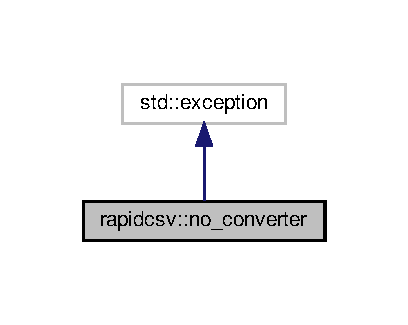
\includegraphics[width=196pt]{classrapidcsv_1_1no__converter__inherit__graph}
\end{center}
\end{figure}


Collaboration diagram for rapidcsv\+:\+:no\+\_\+converter\+:
\nopagebreak
\begin{figure}[H]
\begin{center}
\leavevmode
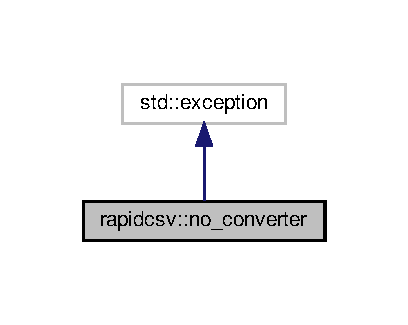
\includegraphics[width=196pt]{classrapidcsv_1_1no__converter__coll__graph}
\end{center}
\end{figure}


\subsection{Detailed Description}
Exception thrown when attempting to access \hyperlink{classrapidcsv_1_1Document}{Document} data in a datatype which is not supported by the \hyperlink{classrapidcsv_1_1Converter}{Converter} class. 

The documentation for this class was generated from the following file\+:\begin{DoxyCompactItemize}
\item 
include/rapidcsv.\+h\end{DoxyCompactItemize}

\hypertarget{structrapidcsv_1_1SeparatorParams}{}\section{rapidcsv\+:\+:Separator\+Params Struct Reference}
\label{structrapidcsv_1_1SeparatorParams}\index{rapidcsv\+::\+Separator\+Params@{rapidcsv\+::\+Separator\+Params}}


Datastructure holding parameters controlling how the C\+SV data fields are separated.  




{\ttfamily \#include $<$rapidcsv.\+h$>$}

\subsection*{Public Member Functions}
\begin{DoxyCompactItemize}
\item 
\hyperlink{structrapidcsv_1_1SeparatorParams_a663909f2406ab233f49f1edea25be505}{Separator\+Params} (const char p\+Separator=\textquotesingle{},\textquotesingle{}, const bool p\+Trim=false, const bool p\+Has\+CR=s\+Platform\+Has\+CR, const bool p\+Quoted\+Linebreaks=false, const bool p\+Auto\+Quote=true)
\begin{DoxyCompactList}\small\item\em Constructor. \end{DoxyCompactList}\end{DoxyCompactItemize}
\subsection*{Public Attributes}
\begin{DoxyCompactItemize}
\item 
\mbox{\Hypertarget{structrapidcsv_1_1SeparatorParams_a8231e02d3e6b917675f30071d39eaebb}\label{structrapidcsv_1_1SeparatorParams_a8231e02d3e6b917675f30071d39eaebb}} 
char \hyperlink{structrapidcsv_1_1SeparatorParams_a8231e02d3e6b917675f30071d39eaebb}{m\+Separator}
\begin{DoxyCompactList}\small\item\em specifies the column separator. \end{DoxyCompactList}\item 
\mbox{\Hypertarget{structrapidcsv_1_1SeparatorParams_a188b1488d2ef5f53e28b156dc9926695}\label{structrapidcsv_1_1SeparatorParams_a188b1488d2ef5f53e28b156dc9926695}} 
bool \hyperlink{structrapidcsv_1_1SeparatorParams_a188b1488d2ef5f53e28b156dc9926695}{m\+Trim}
\begin{DoxyCompactList}\small\item\em specifies whether to trim leading and trailing spaces from cells read. \end{DoxyCompactList}\item 
\mbox{\Hypertarget{structrapidcsv_1_1SeparatorParams_a7f441773d773c69e1ed138164d3d1120}\label{structrapidcsv_1_1SeparatorParams_a7f441773d773c69e1ed138164d3d1120}} 
bool \hyperlink{structrapidcsv_1_1SeparatorParams_a7f441773d773c69e1ed138164d3d1120}{m\+Has\+CR}
\begin{DoxyCompactList}\small\item\em specifies whether new documents should use C\+R/\+LF instead of LF. \end{DoxyCompactList}\item 
\mbox{\Hypertarget{structrapidcsv_1_1SeparatorParams_a0d4cdda7636deba424ed2312fe3c87e0}\label{structrapidcsv_1_1SeparatorParams_a0d4cdda7636deba424ed2312fe3c87e0}} 
bool \hyperlink{structrapidcsv_1_1SeparatorParams_a0d4cdda7636deba424ed2312fe3c87e0}{m\+Quoted\+Linebreaks}
\begin{DoxyCompactList}\small\item\em specifies whether to allow line breaks in quoted text. \end{DoxyCompactList}\item 
\mbox{\Hypertarget{structrapidcsv_1_1SeparatorParams_ae63043bd2471b4ab0c4af34ce042ac47}\label{structrapidcsv_1_1SeparatorParams_ae63043bd2471b4ab0c4af34ce042ac47}} 
bool \hyperlink{structrapidcsv_1_1SeparatorParams_ae63043bd2471b4ab0c4af34ce042ac47}{m\+Auto\+Quote}
\begin{DoxyCompactList}\small\item\em specifies whether to automatically dequote cell data. \end{DoxyCompactList}\end{DoxyCompactItemize}


\subsection{Detailed Description}
Datastructure holding parameters controlling how the C\+SV data fields are separated. 

\subsection{Constructor \& Destructor Documentation}
\mbox{\Hypertarget{structrapidcsv_1_1SeparatorParams_a663909f2406ab233f49f1edea25be505}\label{structrapidcsv_1_1SeparatorParams_a663909f2406ab233f49f1edea25be505}} 
\index{rapidcsv\+::\+Separator\+Params@{rapidcsv\+::\+Separator\+Params}!Separator\+Params@{Separator\+Params}}
\index{Separator\+Params@{Separator\+Params}!rapidcsv\+::\+Separator\+Params@{rapidcsv\+::\+Separator\+Params}}
\subsubsection{\texorpdfstring{Separator\+Params()}{SeparatorParams()}}
{\footnotesize\ttfamily rapidcsv\+::\+Separator\+Params\+::\+Separator\+Params (\begin{DoxyParamCaption}\item[{const char}]{p\+Separator = {\ttfamily \textquotesingle{},\textquotesingle{}},  }\item[{const bool}]{p\+Trim = {\ttfamily false},  }\item[{const bool}]{p\+Has\+CR = {\ttfamily sPlatformHasCR},  }\item[{const bool}]{p\+Quoted\+Linebreaks = {\ttfamily false},  }\item[{const bool}]{p\+Auto\+Quote = {\ttfamily true} }\end{DoxyParamCaption})\hspace{0.3cm}{\ttfamily [inline]}, {\ttfamily [explicit]}}



Constructor. 


\begin{DoxyParams}{Parameters}
{\em p\+Separator} & specifies the column separator (default \textquotesingle{},\textquotesingle{}). \\
\hline
{\em p\+Trim} & specifies whether to trim leading and trailing spaces from cells read (default false). \\
\hline
{\em p\+Has\+CR} & specifies whether a new document (i.\+e. not an existing document read) should use C\+R/\+LF instead of only LF (default is to use standard behavior of underlying platforms -\/ C\+R/\+LF for Win, and LF for others). \\
\hline
{\em p\+Quoted\+Linebreaks} & specifies whether to allow line breaks in quoted text (default false) \\
\hline
{\em p\+Auto\+Quote} & specifies whether to automatically dequote data during read, and add quotes during write (default true). \\
\hline
\end{DoxyParams}


The documentation for this struct was generated from the following file\+:\begin{DoxyCompactItemize}
\item 
include/rapidcsv.\+h\end{DoxyCompactItemize}

%--- End generated contents ---

% Index
\backmatter
\newpage
\phantomsection
\clearemptydoublepage
\addcontentsline{toc}{chapter}{Index}
\printindex

\end{document}
